\documentclass{wissdoc}
% Autor: Roland Bless 1996-2009, bless <at> kit.edu
% ----------------------------------------------------------------
% Hauptdokument
% ----------------------------------------------------------------
%%
%% $Id: thesis.tex 65 2012-05-10 10:32:11Z bless $
%%
%
% Zum Erstellen zweiseitiger PDFs (für Buchdruck) in der Datei "wissdoc.cls" folgende Zeile abändern:
%
% \LoadClass[a4paper,12pt,oneside]{book} % diese Klasse basiert auf ``book''
% in
%\LoadClass[a4paper,12pt,titlepage]{book} % diese Klasse basiert auf ``book''
%
%
% wissdoc Optionen: draft, relaxed, pdf --> siehe wissdoc.cls
% ------------------------------------------------------------------
% Weitere packages: (Dokumentation dazu durch "latex <package>.dtx")
\usepackage[numbers,sort&compress]{natbib}
\usepackage{graphicx}
\usepackage{listings}
\usepackage[ngerman]{babel}

% \usepackage{verbatim}
% \usepackage{float}    %z.B. \floatstyle{ruled}\restylefloat{figure}
% \usepackage{subfigure}
% \usepackage{fancybox} % für schattierte,ovale Boxen etc.
% \usepackage{tabularx} % automatische Spaltenbreite
% \usepackage{supertab} % mehrseitige Tabellen
% \usepackage[svnon,svnfoot]{svnver} % SVN Versionsinformation 
%% ---------------- end of usepackages -------------
%\svnversion{$Id: thesis.tex 65 2012-05-10 10:32:11Z bless $} % In case that you want to include version information in the footer
%% Informationen für die PDF-Datei
\hypersetup{
 pdfauthor={N.N.},
 pdftitle={Not set}
 pdfsubject={Not set},
 pdfkeywords={Not set}
}

% Macros, nicht unbedingt notwendig
%%%%%%%%%%%%%%%%%%%%%%%%%%%%%%%%%%%%%%%%%%%%%%%%%%%%%%%%%%
% macros.tex -- einige mehr oder weniger nuetzliche Makros
% Autor: Roland Bless 1998
%%%%%%%%%%%%%%%%%%%%%%%%%%%%%%%%%%%%%%%%%%%%%%%%%%%%%%%%%%
% $Id: macros.tex 33 2007-01-23 09:00:59Z bless $
%%%%%%%%%%%%%%%%%%%%%%%%%%%%%%%%%%%%%%%%%%%%%%%%%%%%%%%%%%


%%%%%%%%%%%%%%%%%%%%%%%
% Kommentare 
%%%%%%%%%%%%%%%%%%%%%%%
\ifnotdraftelse{
\newcommand{\Kommentar}[1]{}
}{\newcommand{\Kommentar}[1]{{\em #1}}}
% Alles innerhalb von \Hide{} oder \ignore{} 
% wird von LaTeX komplett ignoriert (wie ein Kommentar)
\newcommand{\Hide}[1]{}
\let\ignore\Hide

%%%%%%%%%%%%%%%%%%%%%%%%%
% Leere Seite ohne Seitennummer, wird aber gezaehlt
%%%%%%%%%%%%%%%%%%%%%%%%%

\newcommand{\leereseite}{% Leerseite ohne Seitennummer, nächste Seite rechts (wenn 2-seitig)
 \clearpage{\pagestyle{empty}\cleardoublepage}
}
%%%%%%%%%%%%%%%%%%%%%%%%%%
% Flattersatz rechts und Silbentrennung, Leerraum nach rechts maximal 1cm
%%%%%%%%%%%%%%%%%%%%%%%%%%
\makeatletter
\newcommand{\myraggedright}{%
 \let\\\@centercr\@rightskip 0pt plus 1cm
 \rightskip\@rightskip
  \leftskip\z@skip
  \parindent\z@
  \spaceskip=.3333em
  \xspaceskip=.5em}
\makeatother

\makeatletter
\newcommand{\mynewline}{%
 \@centercr\@rightskip 0pt plus 1cm
}
\makeatother


%%%%%%%%%%%%%%%%%%%%%%%%%%
% Für Index
%%%%%%%%%%%%%%%%%%%%%%%%%%
\makeatletter
\def\mydotfill{\leavevmode\xleaders\hb@xt@ .44em{\hss.\hss}\hfill\kern\z@}
\makeatother
\def\bold#1{{\bfseries #1}}
\newbox\dbox \setbox\dbox=\hbox to .4em{\hss.\hss} % dot box for leaders
\newskip\rrskipb \rrskipb=.5em plus3em % ragged right space before break
\newskip\rrskipa \rrskipa=-.17em plus -3em minus.11em % ditto, after
\newskip\rlskipa \rlskipa=0pt plus3em % ragged left space after break
\newskip\rlskipb \rlskipb=.33em plus-3em minus.11em % ragged left before break
\newskip\lskip \lskip=3.3\wd\dbox plus1fil minus.3\wd\dbox % for leaders
\newskip \lskipa \lskipa=-2.67em plus -3em minus.11em %after leaders
\mathchardef\rlpen=1000 \mathchardef\leadpen=600
\def\rrspace{\nobreak\hskip\rrskipb\penalty0\hskip\rrskipa}
\def\rlspace{\penalty\rlpen\hskip\rlskipb\vadjust{}\nobreak\hskip\rlskipa}
\let\indexbreak\rlspace
\def\raggedurl{\penalty10000 \hskip.5em plus15em \penalty0 \hskip-.17em plus-15em minus.11em}
\def\raggeditems{\nobreak\hskip\rrskipb \penalty\leadpen \hskip\rrskipa %
\vadjust{}\nobreak\leaders\copy\dbox\hskip\lskip %
\kern3em \penalty\leadpen \hskip\lskipa %
\vadjust{}\nobreak\hskip\rlskipa}
\renewcommand*\see[2]{\rlspace\emph{\seename}~#1} % from makeidx.sty

%%%%%%%%%%%%%%%%%%%%%%%%%%
% Neue Seite rechts, leere linke Seite ohne Headings
%%%%%%%%%%%%%%%%%%%%%%%%%%
\newcommand{\xcleardoublepage}
{{\pagestyle{empty}\cleardoublepage}}

%%%%%%%%%%%%%%%%%%%%%%%%%%
% Tabellenspaltentypen (benoetigt colortbl)
%%%%%%%%%%%%%%%%%%%%%%%%%%
\newcommand{\PBS}[1]{\let\temp=\\#1\let\\=\temp}
\newcolumntype{y}{>{\PBS{\raggedright\hspace{0pt}}}p{1.35cm}}
\newcolumntype{z}{>{\PBS{\raggedright\hspace{0pt}}}p{2.5cm}}
\newcolumntype{q}{>{\PBS{\raggedright\hspace{0pt}}}p{6.5cm}}
\newcolumntype{g}{>{\columncolor[gray]{0.8}}c} % Grau
\newcolumntype{G}{>{\columncolor[gray]{0.9}}c} % helleres Grau

%%%%%%%%%%%%%%%%%%%%%%%%%%
% Anführungszeichen oben und unten
%%%%%%%%%%%%%%%%%%%%%%%%%%
\newcommand{\anf}[1]{"`{#1}"'}

%%%%%%%%%%%%%%%%%%%%%%%%%%
% Tiefstellen von Text
%%%%%%%%%%%%%%%%%%%%%%%%%%
% S\tl{0} setzt die 0 unter das S (ohne Mathemodus!)
% zum Hochstellen gibt es uebrigens \textsuperscript
\makeatletter
\DeclareRobustCommand*\textlowerscript[1]{%
  \@textlowerscript{\selectfont#1}}
\def\@textlowerscript#1{%
  {\m@th\ensuremath{_{\mbox{\fontsize\sf@size\z@#1}}}}}
\let\tl\textlowerscript
\let\ts\textsuperscript
\makeatother

%%%%%%%%%%%%%%%%%%%%%%%%%%
% Gauß-Klammern
%%%%%%%%%%%%%%%%%%%%%%%%%%
\newcommand{\ceil}[1]{\lceil{#1}\rceil}
\newcommand{\floor}[1]{\lfloor{#1}\rfloor}

%%%%%%%%%%%%%%%%%%%%%%%%%%
% Average Operator (analog zu min, max)
%%%%%%%%%%%%%%%%%%%%%%%%%%
\def\avg{\mathop{\mathgroup\symoperators avg}}

%%%%%%%%%%%%%%%%%%%%%%%%%%
% Wortabkürzungen
%%%%%%%%%%%%%%%%%%%%%%%%%%
\def\zB{z.\,B.\ }
\def\dh{d.\,h.\ }
\def\ua{u.\,a.\ }
\def\su{s.\,u.\ }
\newcommand{\bzw}{bzw.\ }

%%%%%%%%%%%%%%%%%%%%%%%%%%%%%%%%%%%
% Einbinden von Graphiken
%%%%%%%%%%%%%%%%%%%%%%%%%%%%%%%%%%%
% global scaling factor
\def\gsf{0.9}
%% Graphik, 
%% 3 Argumente: Datei, Label, Unterschrift
\newcommand{\Abbildung}[3]{%
\begin{figure}[tbh] %
\centerline{\scalebox{\gsf}{\includegraphics*{#1}}} %
\caption{#3} %
\label{#2} %
\end{figure} %
}
\let\Abb\Abbildung
%% Abbps
%% Graphik, skaliert, Angabe der Position
%% 5 Argumente: Position, Breite (0 bis 1.0), Datei, Label, Unterschrift
\newcommand{\Abbildungps}[5]{%
\begin{figure}[#1]%
\begin{center}
\scalebox{\gsf}{\includegraphics*[width=#2\textwidth]{#3}}%
\caption{#5}%
\label{#4}%
\end{center}
\end{figure}%
}
\let\Abbps\Abbildungps
%% Graphik, Angabe der Position, frei wählbares Argument für includegraphics
%% 5 Argumente: Position, Optionen, Datei, Label, Unterschrift
\newcommand{\Abbildungpf}[5]{%
\begin{figure}[#1]%
\begin{center}
\scalebox{\gsf}{\includegraphics*[#2]{#3}}%
\caption{#5}%
\label{#4}%
\end{center}
\end{figure}%
}
\let\Abbpf\Abbildungpf

%%
% Anmerkung: \resizebox{x}{y}{box} skaliert die box auf Breite x und Höhe y,
%            ist x oder y ein !, dann wird das usprüngliche 
%            Seitenverhältnis beibehalten.
%            \rescalebox funktioniert ähnlich, nur das dort ein Faktor
%            statt einer Dimension angegeben wird.
%%
% \Abbps{Position}{Breite in Bruchteilen der Textbreite}{Dateiname}{Label}{Bildunterschrift}
%

\newcommand{\refAbb}[1]{%
s.~Abbildung \ref{#1}}

%%%%%%%%%%%%%%%%%%%%
%% end of macros.tex
%%%%%%%%%%%%%%%%%%%%

% Print URLs not in Typewriter Font
\def\UrlFont{\rm}

\newcommand{\blankpage}{% Leerseite ohne Seitennummer, nächste Seite rechts
 \clearpage{\pagestyle{empty}\cleardoublepage}
}

%% Einstellungen für das gesamte Dokument

% Trennhilfen
% Wichtig! 
% Im ngerman-paket sind zusätzlich folgende Trennhinweise enthalten:
% "- = zusätzliche Trennstelle
% "| = Vermeidung von Ligaturen und mögliche Trennung (bsp: Schaf"|fell)
% "~ = Bindestrich an dem keine Trennung erlaubt ist (bsp: bergauf und "~ab)
% "= = Bindestrich bei dem Worte vor und dahinter getrennt werden dürfen
% "" = Trennstelle ohne Erzeugung eines Trennstrichs (bsp: und/""oder)

% Trennhinweise fuer Woerter hier beschreiben
\hyphenation{
% Pro-to-koll-in-stan-zen
}

% Index-Datei öffnen
\ifnotdraft{\makeindex}

\begin{document}

\frontmatter
\pagenumbering{roman}
\ifnotdraft{
 %% Titelseite
%% Vorlage $Id: titelseite.tex 61 2012-05-03 13:58:03Z bless $

\def\usesf{}
\let\usesf\sffamily % diese Zeile auskommentieren für normalen TeX Font

\newsavebox{\Erstgutachter}
\savebox{\Erstgutachter}{\usesf Prof. Dr. Henning Fernau}
\newsavebox{\Zweitgutachter}
\savebox{\Zweitgutachter}{\usesf Petra Wolf}
\newsavebox{\Betreuer}
\savebox{\Betreuer}{\usesf Petra Wolf}

\begin{titlepage}
\setlength{\unitlength}{1pt}
\begin{picture}(0,0)(85,770)
%\includegraphics[width=\paperwidth]{logos/KIT_Deckblatt}
\end{picture}

\thispagestyle{empty}

%\begin{titlepage}
%%\let\footnotesize\small \let\footnoterule\relax
\begin{center}
\hbox{}
\vfill
{\usesf
{\huge\bfseries Implementierung eines historischen Brettspiels in Unity: Latrunculi \par}
\vskip 1.8cm
{\huge Bachelorarbeit}\\
\vskip 0.5cm
zur Erlangung des akademischen Grades\\
Bachelor of Science (B.Sc.) 
\vskip 1.5cm

{\large Universität Trier\\
FB IV - Informatikwissenschaften\\
Professur Theoretische Informatik\\}

\vskip 3cm
\begin{tabular}{p{3.5cm}l}
Gutachter: & \usebox{\Erstgutachter} \\
 & \usebox{\Zweitgutachter} \\
Betreuer: & \usebox{\Betreuer} \\
\end{tabular}
\vskip 3cm
Vorgelegt am xx.xx.xxxx von:\\
\vskip .5cm
Alexander Pet\\
Hohenzollernstraße 3\\
54290 Trier\\
s4alpett@uni-trier.de\\
Matr.-Nr. 1205780


}
\end{center}
\vfill
\end{titlepage}
%% Titelseite Ende


%%% Local Variables: 
%%% mode: latex
%%% TeX-master: "thesis"
%%% End: 

 %\blankpage % Leerseite auf Titelrückseite
 \chapter*{Zusammenfassung}
%% ==============================

In dieser Arbeit wird das Spiel Latrunculi betrachtet und eine digitale Version für das Landesmuseum Birkenfeld umgesetzt. Zum Zeitpunkt dieser Arbeit begleiten uns Kontaktbeschränkungen im Alltag, daher war die Idee dem Museum eine Alternative bieten zu können, die auch online abgerufen werden kann. Daher wurde mit Hilfe der Unity Game Engine eine unter Windows lauffähige Version, sowie eine webbasierte implementiert. Hierzu wurden überlieferte Spielregeln umgesetzt und eigene Ideen für ein Spielende festgelegt, da historisch nicht alle Informationen überliefert wurden. Zur Umsetzung habe ich mich mit dem deterministischen MiniMax-Algorithmus auseinandergesetzt, sowie die Verbesserung Alpha-Beta betrachtet. Diese implementierte künstliche Intelligenz wurde genutzt um das Spielen gegen den Computer zu ermöglichen und zur Simulation bei der zwei KIs gegeneinander antreten. Das Verhalten beider Möglichkeiten wurde im 6. Kapitel analysiert. Bei dieser Analyse hat sich herausgestellt, dass es wenig sinnvoll ist KIs mit den selben Konfigurationen gegeneinander antreten zu lassen. Diese KIs tendieren dazu sich gegenseitig auszuweichen. Weiterhin wurde das Verhalten gegen menschliche Spieler beobachtet und verbessert. Eine primitive Version wurde zu Beginn sehr leicht geschlagen, konnte aber mit einigen Anpassungen in der Analyse der Situation verbessert werden.


%Hier steht eine Kurzzusammenfassung (Abstract) der Arbeit. Stellen Sie kurz und präzise Ziel und Gegenstand der Arbeit, die angewendeten Methoden, sowie die Ergebnisse der Arbeit dar. Halten Sie dabei die ersten Punkten eher kurz und fokussieren Sie die Ergebnisse. Bewerten Sie auch die Ergebnissen und ordnen Sie diese in den Kontext ein.

%Die Kurzzusammenfassung sollte maximal 1 Seite lang sein.

}
%
%% *************** Hier geht's ab ****************
%% ++++++++++++++++++++++++++++++++++++++++++
%% Verzeichnisse
%% ++++++++++++++++++++++++++++++++++++++++++
\ifnotdraft{
{\parskip 0pt\tableofcontents} % toc bitte einzeilig
%\blankpage
\listoffigures
%\blankpage
%\listoftables
%\blankpage
}


%% ++++++++++++++++++++++++++++++++++++++++++
%% Hauptteil
%% ++++++++++++++++++++++++++++++++++++++++++
\graphicspath{{img/}}

\mainmatter
\pagenumbering{arabic}
%% Einleitung.tex
%% $Id: einleitung.tex 61 2012-05-03 13:58:03Z bless $
%%

\chapter{Einleitung}
\label{ch:Latrunculi}
%% ==============================


Die Einleitung besteht aus der Motivation, der Problemstellung, der Zielsetzung und einem erster Überblick über den Aufbau der Arbeit.

%% ==============================
\section{Motivation}
%% ==============================
\label{ch:Einleitung:sec:Motivation}
Da wir uns zum Zeitpunkt der Verfassung dieser Arbeit in einer durch Covid-19 verursachten Pandemie befinden und uns somit Kontaktbeschränkungen im Alltag begleiten, ist die Motivation vor allem den Besuchern des Landesmuseum Birkenfeld ein historisches Spiel online anbieten zu können, da Museumsbesuche nur eingeschränkt möglich sind. Latrunculi wurde implementiert, weil es aufgrund von nicht eindeutig überlieferten Regeln einen gewissen Spielraum in der Umsetzung. Außerdem auch historisch interessante Informationen liefert. Weiterhin bietet das Landesmuseum Birkenfeld Veranstaltungen (https://www.landesmuseum-birkenfeld.de/landesmuseum/erlebnismuseum/), wie ,,So spielten die Römer'' für Schulklassen an und kann durch eine digitale und spielbare Umsetzung  eines historischen Spiels bei den Besuchern ein größeres Interesse wecken.
%Zugang einfacher!


%%Warum ist das zu bearbeitende Themengebiet spannend und relevant?

%% ==============================
%%\section{Variationen?}
%% ==============================
%%\label{ch:Einleitung:sec:Problemstellung}

%%Welches Problem/welche Probleme können in diesem Themengebiet identifiziert werden?

%% ==============================
\section{Problemstellung}
%% ==============================
\label{ch:Einleitung:sec:Problemstellung}
Latrunculi war historisch gesehen ein beliebtes und weit verbreitetes strategisches Brettspiel der Römer und Griechen gewesen sein. Die römischen Dichter Ovid und Martial haben dieses Spiel bereits erwähnt und beschrieben, dass bei sehr talentierten Spielern häufig Zuschauer anwesend waren. Die Spielsteine wurden als latrones(lat. für Soldat) bezeichnet. Da die Entstehung dieses Spiels so lange zurück liegt, wurden nicht alle Regeln überliefert, sodass verschieden Quellen hinzugezogen werden müssen um den Spielmechanismen zu klären. Das Latrunculi-Spielfeld besteht aus einem Raster senkrechter und waagerechter Reihen. Weiterhin wurden wahrscheinlich die Spielsteine auf den Feldern und nicht auf den Linien platziert und bewegt. Dabei konnte keine fixe Größe des Spielbretts festgestellt werden, sodass verschieden große Spielfelder mit unterschiedlicher Anzahl an Zellen gefunden wurden. Bei Ausgrabungen konnten Latrunculi-Bretter mit beispielsweise 7x7, 8x8, 9x10, 7x10 und 7x6 Feldern geborgen werden. Als Spielbretter dienten hierbei unter anderem Kalksteine oder Ziegelsteine, wie sie in Mainz oder in Hadrianswall in Großbritannien gefunden wurden. Betrachtet man Ovids Aussagen, kann man folgern, dass das Hauptziel darin bestand mit seinen Spielsteinen einen gegnerischen von zwei gegenüberliegenden Seiten zu einzufangen und somit aus dem Spiel zu nehmen. Weiterhin beschreibt er, dass es wichtig sei, seine Steine paarweise zu bewegen, da dadurch verhindert wird, dass diese vom Gegner geschlagen werden können. Für diesen Angriffs- und Verteidigungsmechanismus konnten die Steine geradlinig vorwärts und rückwärts verschoben werden. Allerdings ist auch nicht eindeutig erklärt, wann das Spiel endet oder ob es mit speziellen Figuren funktioniert hat, beispielsweise gibt es Variationen mit einem König mit speziellen Fähigkeiten, ähnlich wie die Dame beim Schach, zwischen den simplen Figuren beziehungsweise Steinen.

%% ==============================
\section{Zielsetzung}
%% ==============================
\label{ch:Einleitung:sec:Zielsetzung}
In dieser Arbeit wird eine nachfolgend erklärte Variation des Spiels Latrunculi mithilfe der Unity Engine für das Landesmuseum Birkenfeld umgesetzt. Dabei wurde eine Künstliche Intelligenz implementiert, sodass es die Möglichkeit gibt, gegen eine KI zu spielen, die zielführende Züge umsetzt. Weiterhin soll das entwickelte Spiel die Möglichkeit bieten, zwei KI's als Simulation gegeneinander antreten zu lassen. Zum Zeitpunkt der Arbeit, befinden wir uns aufgrund von Covid-19 in einer Pandemie, sodass aktuell Kontaktbeschränkungen den Alltag bestimmen, daher soll das Projekt auch die Möglichkeit bieten online abgerufen zu werden. Unity bietet relativ einfache Portierungs-Möglichkeiten, sodass die Entwicklung eines Spiels für unterschiedliche Plattformen erleichtert wird.


%% Was ist das Ziel der Arbeit. Wie soll das Problem gelöst werden?


%% ==============================
\section{Gliederung/Aufbau der Arbeit}
%% ==============================
\label{ch:Einleitung:sec:Gliederung}

%%Was enthalten die weiteren Kapitel? Wie ist die Arbeit aufgebaut? Welche Methodik wird verfolgt?

Die folgenden Kapitel behandeln zuerst die Grundlagen, um die anschließend aufgeführten Abschnitte besser verstehen zu können. Dabei werden die umgesetzten Spielregeln erklärt, sowie die grundsätzliche Definition von Künstlicher Intelligenz, als auch Umsetzungen in bekannten Spielen erwähnt. Außerdem wird die Engine Unity kurz erklärt und der verwendete Algorithmus für die künstliche Intelligenz. Das Dritte Kapitel umfasst sowohl die technischen Anforderungen, als auch nötige Funktionalitäten des Spiels.
Im Anschluss an den dritten Abschnitt wird das Konzept, die nötigen Features und Technologien beschrieben.
Das 5. Kapitel erklärt die Implementierung des Spiels, sowie der KI. Anschließend wird erklärt, wie der Release beim Kunden im Museum unter gegebenen Umständen stattgefunden hat.

%%% Local Variables: 
%%% mode: latex
%%% TeX-master: "thesis"
%%% End: 
  % Einleitung
%% grundlagen.tex
%% $Id: grundlagen.tex 61 2012-05-03 13:58:03Z bless $
%%

\chapter{Grundlagen}
\label{ch:Grundlagen}
%% ==============================

%% ==============================
\section{Spielregeln}
%% ==============================
\label{ch:Grundlagen:sec:Abschnitt1}
Der grundsätzliche Aufbau des Spiels beinhaltet ein Spielbrett mit beispielsweise 7x6 Feldern bis hin zu überlieferten 12x12 großen Brettern. Weiterhin gibt es zwei verschiedene Spielsteine, die entweder unterschiedliche Farben haben oder aus zum Beispiel einerseits Steinen und andererseits Muscheln, wie in dieser Ausarbeitung auch, bestehen. Dabei übernimmt ein Spieler die Steine und der Gegenspieler die Muscheln. Zu Beginn werden die eigenen Steine jeweils auf der ersten Reihe  platziert (Abbildung \ref{fig:startzustand}).
\\

\begin{figure}[h]
	\centering
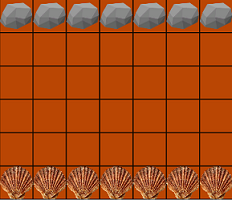
\includegraphics{img/regeln_startzustand2}
\caption{Startkonfiguration eines 7x6 Latrunculi Feldes}
\label{fig:startzustand}
\end{figure}

Das Spiel beginnt mit einem der beiden Spieler. Während des Spiels ziehen die Spieler abwechselnd horizontal oder vertikal über das Feld, ohne dabei einen anderen Stein zu überspringen oder auf einer besetzten Zelle zu landen (Abbildungen \ref{fig:Bewegungen} \& \ref{fig:nottodo}).


\begin{figure}[h]
	\centering
	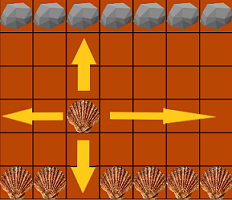
\includegraphics{img/regeln_bewegung22}
	\caption{Legitime Bewegungen}
	\label{fig:Bewegungen}
\end{figure}

\begin{figure}[h]
	\centering
	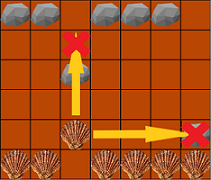
\includegraphics{img/regeln_nottodo2}
	\caption{nicht zulässige Bewegung}
	\label{fig:nottodo}
\end{figure}

Um gegnerische Spielsteine zu erobern, müssen diese wie in der Abbildung \ref{fig:erobern} von eigenen Steinen auf zwei gegenüberliegenden Feldern umstellt sein.


\begin{figure}[h]
	\centering
	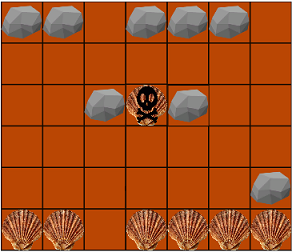
\includegraphics{img/regeln_erobern2}
	\caption{Erobern}
	\label{fig:erobern}
\end{figure}


Wird ein gegnerischer Stein erobert, dann wird dieser aus dem Spiel entfernt und ein eigener darf nochmal bewegt werden. Hierbei gibt es auch Variationen bei denen nur der zuletzt bewegte Stein sich wieder bewegen darf.
Bewegt sich ein eigener Stein zwischen zwei gegnerische und scheint somit umstellt zu sein, zählt dieser allerdings nicht als erobert(Abbildung \ref{fig:nichterobern}).
\begin{figure}[h]
	\centering
	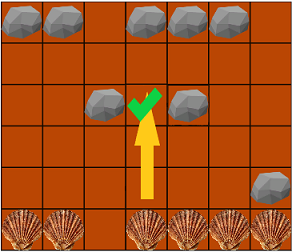
\includegraphics{img/regeln_nichterobert2}
	\caption{Keine Eroberung}
	\label{fig:nichterobern}
\end{figure}

Das Ziel des Spiels ist es, dass der Gegenspieler keinen Zug mehr ausführen kann beziehungsweise keinen Spielstein mehr erobern kann.


%% ==============================
%\section{Künstliche Intelligenz}
%% ==============================
%\label{ch:Grundlagen:sec:Abschnitt2}
%\nocite{computerweekly}
%\nocite{barr2014handbook}

%Der amerikanische Informatiker John McCarthy prägte 1956 den Begriff künstliche Intelligenz (KI) auf der Dartmouth Conference.
%Künstliche Intelligenz findet heutzutage in vielen Bereichen Anwendung und ist eine immer wichtigere Entwicklung, um menschliche Arbeit zu vereinfachen und auch auf Computer zu übertragen. Seit der Begriff geprägt wurde, haben sich die dazugehörigen Bereiche erweitert. Heute definiert KI die Automatisierung von Prozessen bis hin zur Robotik.
%Hierbei geht es vor allem um den Zusammenhang zwischen Berechnung und Wahrnehmung.
%Aufgrund der riesigen Datenmengen (Big Data), die ein Mensch alleine nicht bearbeiten oder analysieren kann, wird dieser Bereich immer wichtiger. Maschinen können viel effizienter Daten analysieren und Muster erkennen, als ein Mensch es könnte.\\
%Um die unterschiedlichen Typen zu kategorisieren, kann man sich die vier verschiedenen Typen, die von Arend Hintze, Assistenzprofessor für Integrative Biologie und Informatik der Michigan State University klassifiziert wurden, betrachten:

%\paragraph{Typ 1: Reaktive Maschinen}
%Zu den Reaktiven Maschinen zählen solche, die den aktuellen Zustand kennen und zukünftige Entscheidungen analysieren und bewerten können. Als Beispiel kann man sich hier Deep Blue anschauen. Deep Blue ist ein von IBM entwickeltes Schachprogramm und ist in der Lage die Figuren auf dem Spielbrett zu erkennen  und mögliche Züge beider Spieler analysieren. Da Deep Blue keine lernende Komponente enthält, werden vergangenen Spielsituationen nicht betrachtet und haben keinen Einfluss auf zukünftige Züge.

%\paragraph{Typ 2: Begrenzter Speicher}
%Zum zweiten Typen zählt man Systeme, die vergangene Erfahrungen nutzen können, allerdings werden hier Beobachtungen aus naher Zukunft nicht gespeichert. Als Beispiel können hier autonome Fahrzeuge betrachtet werden, die den Wechsel der Fahrspur eines Autos nicht dauerhaft speichern.\\
%\newline
%Die nachfolgenden beiden Typen existieren in der beschriebenen Form noch nicht:
%\paragraph{Typ 3: Native Theorie}
%Die Native Theorie ist ein psychologischer Begriff und bezeichnet Systeme, die verstehen, dass andere eigene Überzeugungen, Wünsche und Absichten haben, die ihre Entscheidungen beeinflussen.
%\paragraph{Typ 4: Selbsterkenntnis}
%Diese Kategorie umfasst Maschinen die ein Bewusstsein haben.Die sollen in der Lage sein ihren aktuellen Zustand zu verstehen und daraus Erkenntnisse über das Gefühl anderer zu ziehen.\\
%\newline
%In dieser Ausarbeitung wurde im Zusammenhang mit dem Spiel Latrunculi eine künstliche Intelligenz des Typ 1 entwickelt, die ihren aktuellen Zustand kennt und daraus Berechnungen für zukünftige Züge treffen kann.
%% ==============================
%\subsection{Künstliche Intelligenz in Videospielen}
%% ==============================
%\label{ch:Grundlagen:sec:Abschnitt3}
%\nocite{tecchannel}
%In Videospielen werden in der Regel Reaktive Maschinen verwendet. Hierbei werden mögliche Bewegungen entweder vorher definiert und abgearbeitet oder aber die Aktionen werden mit einem Punktesystem bewertet und abhängig von der Punktzahl ausgeführt. Dabei lässt sich festhalten, dass je mehr Bewertungskriterien die Aktionen bekommen, desto intelligenter wirkt die Künstliche Intelligenz. Betrachtet man die Entwicklung der Videospiele der letzten Jahre im Allgemeinen, fällt auf, dass vor Allem die Grafik weite Sprünge gemacht hat, im Vergleich dazu aber die eingesetzte KI sich nicht wesentlich verändert hat.\\
%Als Beispiel kann man sich das Strategiespiel Command \& Conquer aus dem Jahre 1996 anschauen, sowie den Nachfolger Command \& Conquer (2007) erkennt man das Problem das sich hier abzeichnet. Während sich die Grafik innerhalb der 11 Jahre wesentlich verbessert hat, verhält sich die KI noch immer ähnlich und es passieren die selben Fehler wie schon beim ersten Teil. Spieler müssen in diesem Spiel ein Hauptquartier aufbauen und von diesem aus die gegnerischen Spieler ausschalten, dabei müssen Rohstoffe gesammelt werden um die Basis weiter auszubauen. Zur Rohstoffgewinnung verfügt man über so genannte Ernter, welche automatisch den Rohstoff Tiberium suchen. Bei der Suche fahren diese teilweise ins gegnerische Hauptquartier und werden dort zerstört. Im Nachfolger, elf Jahre später, verhalten sich die Ernter noch immer ähnlich und die Fehler passieren hier ebenfalls, allerdings mit dem Unterschied, dass das Spiel, der Ernter und die Explosions-Animation grafisch realistischer aussehen. Wenn man hier eine lernende Komponente implementieren würde, dann könnten solche Probleme der KI zwar noch passieren, aber auf Dauer wäre Sie in der Lage, das als Fehler zu erkennen. \\

%\paragraph{MiniMax-Algorithmus}
%Der Minimax-Algorithmus dient der Entscheidungsfindung eines optimalen Spielzuges vor allem in Zwei-Spieler Spielen wie Schach oder Backgammon bei denen sich die Spieler mit ihren Zügen abwechseln. Effizient angewendet werden kann der Algorithmus vor Allem in \textbf{Nullsummenspielen}.\\
%Ein Spiel ist ein \textbf{Nullsummenspiel}, wenn die Summe aus Gewinnn und Verlust aller Spieler nach Spielende Null ergibt, das heißt der Gewinn eines Spielers ist der Verlust beziehungsweise die Niederlage eines anderen.\cite{AlphaBeta}.\\
%Diesen Algorithmus kann man sich als Spielbaum vorstellen, der mit jedem Pfad einen denkbaren Spielverlauf darstellt. Dabei repräsentiert jeder Knoten des Baumes einen Spielzustand und enthält Informationen über die Verteilung der Figuren auf dem Spielbrett, welcher Spieler am Zug ist und über mögliche weitere Spielzüge. Jeder dieser Züge ist ebenfalls wieder ein Knoten und Kind der vorherigen Aktion.

%\subparagraph{Beispiel 2.1:}
%Am einfachsten kann man sich die Funktionsweise am Beispiel von TicTacToe klar machen:\\
%Dabei repräsentiert wieder jeder Knoten, der hier als Abbildung des Spielbretts dargestellt wird, einen Zustand des Spiels. Die Bewertung der Zustände ist in diesem Spiel vergleichsweise simpel:\\
%\begin{itemize}
%	\item Spieler 1 gewinnt: +1 Punkt,
%	\item Unentschieden: 0 Punkte,
%	\item Spieler 2 gewinnt: -1 Punkt
%\end{itemize}
%\begin{figure}[h]
%	\centering
%	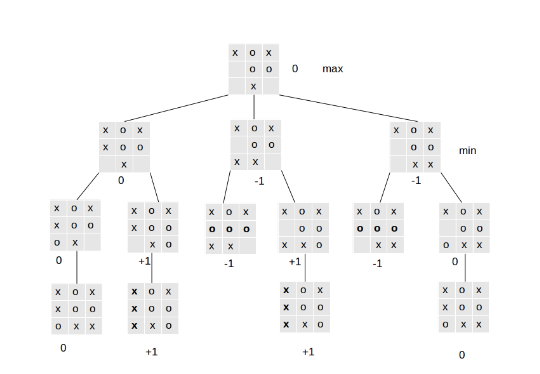
\includegraphics{img/Baum}
%	\caption{TicTacToe Spielbaum}
%	\cite{AlphaBeta}
%	\label{fig:Suchbaum}
%\end{figure}
%Der Algorithmus basiert auf der Idee, anhand dieses Baumes den Verlauf mit dem höchsten Wert zu verfolgen und so das Spiel zu gewinnnen. Dabei wird wie in Abbildung \ref{fig:Suchbaum} zu sehen, jedem Knoten ein Wert zugeordnet und versucht immer den höchstmöglichen Wert zu erzielen, wenn der Spieler gewinnen soll.

%\paragraph{Analyse \& Variationen}
%Aufgrund von tendenziell hoher Laufzeit, vor Allem bei komplexeren Spielen, gibt es verschiedene Variationen dieses Algorithmus.
%In der Basis-Version des MiniMax enden die möglichen Verläufe im ungünstigsten Fall nach $d$ Zügen, wobei $d$ für die Suchtiefe im Baum steht. Im extremsten Fall können wir annehmen, dass aus jedem Zustand weitere $w$ Züge möglich sind. Daraus resultieren auf der untersten Ebene $ w ^d$ Knoten und es gilt \[ \sum_{i=1}^d  w^{d}\in O(w^d).\]\\
%Zur Optimierung existieren unterschiedliche Variationen von denen eine hier näher beschrieben wird.
%\paragraph{Alpha-Beta-Algorithmus}
%Aufgrund der hohen Komplexität wird auch der \textbf{Alpha-Beta-Algorithmus} verwendet. Dieser basiert auf dem MiniMax-Algorithmus, allerdings wird hier der Wert der möglichen Endzustände geschätzt und die Berechnnung eines Pfads abgebrochen, sobald klar ist, dass dieser Weg weniger zielführend ist. Dabei wird angenommen, dass Zweige ab einem Punkt in der Berechnung vernachlässigt werden können. Am nachfolgenden Beispiel wird die Idee deutlicher:
%\subparagraph{Beispiel 2.2:}
%Nach der Durchsuchung des linken Teilbaums, sieht man, dass der der Ausgangsknoten mindestens den Wert 3 hat. Deshalb wird die Evaluation des rechten Teilbaums abgebrochen, sobald klar wird, dass der min-Knoten maximal einen Wert von 2 hat. Die Suche kann abgebrochen werde, da der rechte Teilbaum keine Auswirkungen auf den Startknoten hat\nocite{AlphaBeta}.
%\begin{figure}[h]
%	\centering
%	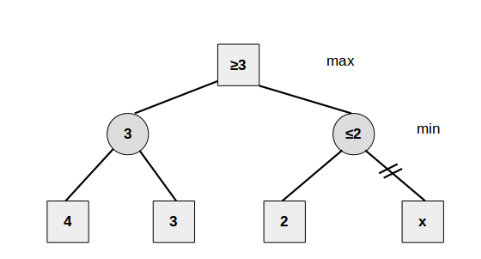
\includegraphics{img/AlphaBeta}
%	\caption{Alpha-Beta Spielbaum}
%	\cite{AlphaBeta}
%	\label{fig:AlphaBeta}
%\end{figure}
%% ==============================
\section{Unity Engine}
%% ==============================
\label{ch:Grundlagen:sec:Unity}
\nocite{ConceptArt}

Die Unity Engine ist eine von Unity Technologies entwickelte Laufzeit- und Entwicklungsumgebung für Videospiele. Die Engine bietet dabei Portierungen für PCs, Spielkonsolen, mobile Geräte wie Android und Webbrowser. Bekannte Spiele wie Pokemon Go und Hearthstone wurden mit Unity entwickelt. Weiterhin bietet Unity die Möglichkeit sowohl in 2D als auch in 3D Spiele umzusetzen und bietet Funktionen, wie den Eventhandler für Gameobjects um die Entwicklung zu vereinfachen. Um selbstgeschriebene Scripte einzubinden unterstützt Unity unter anderem C\#, wie ich es in dieser Arbeit auch verwendet habe. Unity wurde hier vor allem wegen der einfachen Portierung und Wiederverwendbarkeit von vorgefertigt erstellten Prefabs genutzt. Ausserdem bietet Unity eine große Anzahl an Libraries zur Unterstützung der Spielentwicklung. \\Unity bietet die Möglichkeit einerseits per Drag \& Drop Spielobjekte im Editor zu platzieren und diesen Objekten so ihren Ausgangszustand zu geben. Außerdem besteht die Möglichkeit die Szene dynamisch via Skript zu erstellen. Entwickelt man in der 2D Umgebung, hat man die Möglichkeit seinen Objekten Sprites mitzugeben. Diese Sprites sind Grafikobjekte die als Darstellung der Spielobjekte im Editor platziert werden. In einem Unity Projekt befindet sich ein Ordner ,,Assets'' in dem alle selbst erstellten Skripte, Sprites und Szenen enthalten sind, sowie andere genutzte Ressourcen wie zuvor erstellte Prefabs für eine dynamische Generierung.

\paragraph{Prefab System}
\nocite{UPrefabs}
Unitys Prefab System ermöglicht es Spielobjekte zu erstellen und als Prefab zu speichern. Diese Prefabs können wiederverwendet werden und fungieren wie ein Vorlage(Template) eines Objektes. Dadurch können wiederkehrende Spielobjekte einmalig definiert werden und durch das Prefab in der selben Form oder aber auch verändert mehrfach genutzt werden. Das heißt es können dadurch zur Laufzeit Spielobjekte instanziiert und zur Szene hinzugefügt werden ohne jedes einzelne Objekt neu zu definieren. Weiterhin können diese so erstellten Objekte trotzdem noch separat verändert werden.

%% ==============================
\section{Künstliche Intelligenz}
%% ==============================#
\label{ch:Grundlagen:sec:Künstliche Intelligenz}
Allgemein kann man sagen, dass es drei Formen der künstlichen Intelligenz gibt. Zum einen sollte man zwischen deterministischen und strategischen KIs unterscheiden, andererseits kann man diese vom Machine und Deep Lerning abgrenzen.

\subsection{Strategische KIs}
\label{ch:Grundlagen:sec:strategisch}
\textbf{Strategische KIs} werden in Videospielen zum Beispiel zur Wegfindung oder für die Atmosphäre genutzt. Am Beispiel von sogenannten Non-Player-Character (kurz:NPC) in Rollenspielen wie Gothic kann diese Form  gut erklärt werden. NPCs sind Figuren innerhalb eines Spiels mit denen in der Regel interagiert werden kann oder die für die Atmosphäre eingesetzt werden und nur einen Weg ablaufen, der via Wegfinde-Algorithmus berechnet wird. Außerdem kann auch das Verhalten beeinflusst werden, indem die Spielfiguren auf Aktionen reagieren können und in einen entsprechenden Zustand versetzt werden. Betrachtet man das Spiel Gothic, erkennt man sehr leicht dieses Prinzip. Hier ist es möglich, dass der Spieler durch sein Verhalten die NPCs beeinflusst. Es existieren Figuren, die einem aggressiv gegenübertreten, falls man zum Beispiel zuvor aus seinem Haus etwas geklaut hat. Für diese NPCs werden strategische KIs eingesetzt, um vor allem die Handlung zu unterstützen.

\subsection{Deterministische KIs}
\label{ch:Grundlagen:sec:deterministisch}
\textbf{Deterministische KIs} können Anwendung in Brettspielen finden. Hier werden Algorithmen verwendet um den Spielzustand und zukünftige zu bewerten und daraus die optimale Aktion zu finden. Diese Systeme können als Baumstruktur dargestellt werden. In dieser Arbeit wurde beispielsweise der MinMax-Algorithmus implementiert.

\paragraph{MinMax}
Beim MinMax-Algorithmus entspricht der Ausgangsknoten dem aktuellen Zustand und jedes Kind steht für einen zukünftigen. Diese Zustände werden nach verschiedenen Kriterien bewertet und so eine Punktzahl für jeden Zustand errechnet. An der Abbildung \ref{fig:Spielbaum} wird das Prinzip deutlicher. Dabei ist im Ausgangszustand Spieler 1 an der Reihe gewesen. Die drei abgebildeten Kinder sind jeweils mögliche Züge des zweiten Spielers. Der linke Zustand hat die Wertung 0, da hier weder eine Bedrohung oder ein Abzug aus einer Bedrohung, noch ein Angriff stattfindet. Die beiden anderen Kinder haben eine Wertung von +30, da diese Zustände zu einer Bedrohung der Muscheln führen. Die nächste Reihe zeigt mögliche Züge der Steine, die aus den vorherigen Situationen resultieren. Dabei werden Züge mit 40 bewertet, falls eine Muschel sich neben die bedrohte Muschel stellt und diese dadurch vor einer Eroberung schützt. Die höchste Bewertung 100 erhalten die Züge, die den gegnerischen Stein erobern. Diese Bewertungen werden von den höchsten Punktzahlen ausgehend bis zum Ausgangsknoten aufsummiert und ergeben dabei eine Höchstpunktzahl von -40 bei einer Suchtiefe von 2. %In diesem Fall gibt es zwei mögliche Pfade mit der höchsten Wertung. %Also muss für eine Entscheidung noch ein Zufallsgenerator eingesetzt werden der zwischen den beiden möglichen Zügen entscheidet.

\begin{figure}[h]
	\centering
	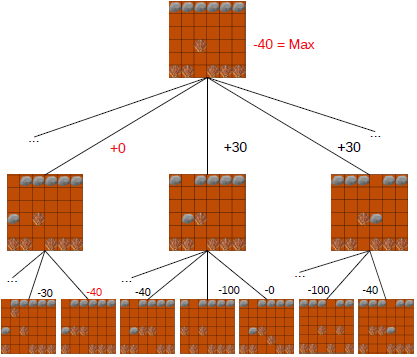
\includegraphics{img/Spielbaum_latrun4}
	\caption{ Ausschnitt: MinMax-Spielbaum eines 6x6 Latrunculi Feldes}
	\label{fig:Spielbaum}
\end{figure}

\subsection{Machine Learning}
\label{ch:Grundlagen:sec:Learning}
Beim Machine Learning wird eine statistische Wissenbasis aufgebaut indem das System mit Daten trainiert wird. Es ist ein Verfahren, dass Algorithmen nutzt um Daten zu analysieren und zu kategorisieren. Als Beispiel kann die Gesichtserkennung genannt werden. Hier werden die Systeme mit unterschiedlichen Gesichtern trainiert um anschließend diese erkennen und zuordnen zu können. Generell kann man festhalten, dass diese Verfahren eher nicht in Videospielen angewendet werden. Es lässt sich zwischen dem Supervised Learning (überwachtes Lernen) und dem unsupervised Learning (nicht überwachtes Lernen).
\paragraph{Supervised Learning}
Das überwachte Lernen funktioniert so, dass ein Algorithmus Trainingsdaten erhält, sowie die Bedeutung der Daten. Dadurch soll der Algorithmus Muster erkennen und in einer Funktion speichern um anschließend diese Muster auf neuen Daten erkennen zu können. Diese Funktion wird abhängig von der Trefferquote vom System angepasst.
\paragraph{Unsupervised Learning}
Beim nicht überwachten Lernen werden nicht kategorisierte Daten dem Algorithmus übergeben, sodass dieser Cluster erkennen soll und zukünftige Daten einordnen kann.\\

%\paragraph{Reinforcement Learning}


%Die künstliche Intelligenz in digitalen Brettspielen funktioniert mit einem Bewertungssystem, dabei kalkuliert man die möglichen Züge. Dieses Ranking wird dann mit entsprechenden Algorithmen wie dem MinMax evaluiert. Diese kann man sich wie einen Baum vorstellen (Abbildung \textbf{TODO}). Dabei entspricht jeder Knoten einem Spielzustand und berechnet je nach festgelegter Tiefe mögliche Verläufe. Für die Bewertung müssen sinnvolle Kriterien festgelegt werden um entscheiden zu können ob der betrachtete Zug einen Spielvorteil bringt. 


%% ==============================
%%\section{State of the Art}
%% ==============================
%\label{ch:Grundlagen:sec:SOTA}
%Die Literaturrecherche soll so vollständig wie möglich sein und bereits existierende relevante Ansätze (Verwandte Arbeiten / State of the Art / Stand der Technik) beschreiben bzw. kurz vorstellen.
%Es soll aufgezeigt werden, wo diese Ansätze Defizite aufweisen oder nicht anwendbar sind, z.B. weil sie von anderen Umgebungen oder Voraussetzungen ausgehen.

%Je nach Art der Abschlussarbeit kann es auch sinnvoll sein, diesen Abschnitt in die Einleitung zu integrieren oder als eigenes Kapitel aufzuführen.

%%Beispiel, wie mit LaTeX zitiert werden kann: \cite{TB98,JSAC96,qosr} \cite{AlphaBeta}

%%% Local Variables: 
%%% mode: latex
%%% TeX-master: "thesis"
%%% End: 
  % Grundlagen
%% analyse.tex
%% $Id: analyse.tex 61 2012-05-03 13:58:03Z bless $

\chapter{Analyse}
\label{ch:Analyse}
%% ==============================
In diesem Kapitel sollen zunächst das zu lösende Problem
sowie die Anforderungen und die Randbedingungen 
einer Lösung\index{Lösung} beschrieben werden (eine präzisierte Aufgabenstellung\index{Aufgabenstellung}).


%% ==============================
\section{Anforderungen}
%% ==============================
\label{ch:Analyse:sec:Anforderungen}
Anforderungen und Randbedingungen\index{Randbedingungen} \ldots

%% ==============================
\section{Weiterer Abschnitt}
%% ==============================
\label{ch:Analyse:sec:Abschnitt}

Lorem ipsum dolor sit amet, consetetur sadipscing elitr, sed diam nonumy eirmod tempor invidunt ut labore et dolore magna aliquyam erat, sed diam voluptua. At vero eos et accusam et justo duo dolores et ea rebum. Stet clita kasd gubergren, no sea takimata sanctus est Lorem ipsum dolor sit amet.

\begin{figure}[htb]
\centering
  	{
\includegraphics[width=.3\textwidth]{Logo-Uni-Trier.jpg}}
	\caption{Logo der Universität Trier.\label{fig:grafik1}}
\centering
\end{figure}

Lorem ipsum dolor sit amet, consetetur sadipscing elitr, sed diam nonumy eirmod tempor invidunt ut labore et dolore magna aliquyam erat, sed diam voluptua. 

\begin{table}[htb]
\caption{Tabelle mit Werten.\label{tab:liste}}
\vspace*{1em}
\centering

\bgroup
\def\arraystretch{1.3}%  1 is the default, change whatever you need

\begin{tabular}[c]{l|l|c}
	
	\multicolumn{1}{c|}{\textbf{A}} & 
	\multicolumn{1}{c|}{\textbf{B}} & 
	\multicolumn{1}{c}{\textbf{C}} \\ 
	
	\hline

	Test 1& Slow& 279 \\ 
	&Fast & 499 \\ 
	&Very fast& 719 \\ 
	
\end{tabular}

\egroup

\end{table}

Duis autem vel eum iriure dolor in hendrerit in vulputate velit esse molestie consequat, vel illum dolore eu feugiat nulla facilisis at vero eros et accumsan et iusto odio dignissim qui blandit praesent luptatum zzril delenit augue duis dolore te feugait nulla facilisi. 

Duis autem vel eum iriure dolor in hendrerit in vulputate velit esse molestie consequat, vel illum dolore eu feugiat nulla facilisis. 

%% ==============================
\section{Zusammenfassung}
%% ==============================
\label{ch:Analyse:sec:zusammenfassung}

Am Ende sollten ggf. die wichtigsten Ergebnisse nochmal in \emph{einem}
kurzen Absatz zusammengefasst werden.

%%% Local Variables: 
%%% mode: latex
%%% TeX-master: "thesis"
%%% End: 
     % Analyse
%% entwurf.tex
%% $Id: entwurf.tex 61 2012-05-03 13:58:03Z bless $
%%

\chapter{Entwurf / Konzeption}
\label{ch:Entwurf}
%% ==============================
In diesem Kapitel erfolgt die ausführliche Beschreibung des eigenen
Lösungsansatzes. Dabei sollten Lösungsalternativen diskutiert und
Entwurfsentscheidungen dargelegt werden.

%% ==============================
\section{Abschnitt 1}
%% ==============================
\label{ch:Entwurf:sec:Abschnitt1}

Lorem ipsum dolor sit amet, consetetur sadipscing elitr, sed diam nonumy eirmod tempor invidunt ut labore et dolore magna aliquyam erat, sed diam voluptua. At vero eos et accusam et justo duo dolores et ea rebum. Stet clita kasd gubergren, no sea takimata sanctus est Lorem ipsum dolor sit amet. Lorem ipsum dolor sit amet, consetetur sadipscing elitr, sed diam nonumy eirmod tempor invidunt ut labore et dolore magna aliquyam erat, sed diam voluptua. At vero eos et accusam et justo duo dolores et ea rebum. Stet clita kasd gubergren, no sea takimata sanctus est Lorem ipsum dolor sit amet. Lorem ipsum dolor sit amet, consetetur sadipscing elitr, sed diam nonumy eirmod tempor invidunt ut labore et dolore magna aliquyam erat, sed diam voluptua. At vero eos et accusam et justo duo dolores et ea rebum. Stet clita kasd gubergren, no sea takimata sanctus est Lorem ipsum dolor sit amet. 

%% ==============================
\section{Abschnitt 2}
%% ==============================
\label{ch:Entwurf:sec:Abschnitt2}

Lorem ipsum dolor sit amet, consetetur sadipscing elitr, sed diam nonumy eirmod tempor invidunt ut labore et dolore magna aliquyam erat, sed diam voluptua. At vero eos et accusam et justo duo dolores et ea rebum. Stet clita kasd gubergren, no sea takimata sanctus est Lorem ipsum dolor sit amet. Lorem ipsum dolor sit amet, consetetur sadipscing elitr, sed diam nonumy eirmod tempor invidunt ut labore et dolore magna aliquyam erat, sed diam voluptua. At vero eos et accusam et justo duo dolores et ea rebum. Stet clita kasd gubergren, no sea takimata sanctus est Lorem ipsum dolor sit amet. Lorem ipsum dolor sit amet, consetetur sadipscing elitr, sed diam nonumy eirmod tempor invidunt ut labore et dolore magna aliquyam erat, sed diam voluptua. At vero eos et accusam et justo duo dolores et ea rebum. Stet clita kasd gubergren, no sea takimata sanctus est Lorem ipsum dolor sit amet. 

Duis autem vel eum iriure dolor in hendrerit in vulputate velit esse molestie consequat, vel illum dolore eu feugiat nulla facilisis at vero eros et accumsan et iusto odio dignissim qui blandit praesent luptatum zzril delenit augue duis dolore te feugait nulla facilisi. Lorem ipsum dolor sit amet, consectetuer adipiscing elit, sed diam nonummy nibh euismod tincidunt ut laoreet dolore magna aliquam erat volutpat. 

%% ==============================
\section{Zusammenfassung}
%% ==============================
\label{ch:Entwurf:sec:zusammenfassung}

Am Ende sollten ggf. die wichtigsten Ergebnisse nochmal in \emph{einem}
kurzen Absatz zusammengefasst werden.

%%% Local Variables: 
%%% mode: latex
%%% TeX-master: "thesis"
%%% End: 
     % Entwurf
%% implemen.tex
%% $Id: implemen.tex 61 2012-05-03 13:58:03Z bless $
%%

\chapter{Implementierung}
\label{ch:Implementierung}
%% ==============================

Aufgrund der unterstützenden Funktionen, wie das Portieren auf verschiedene Systeme, habe ich mich für die Unity Engine in der Version 2019.3.14f entschieden, um Latrunculi digital umzusetzen. Die Erklärung zu Unity befindet sich im Abschnitt \ref{ch:Grundlagen:sec:Unity}. Weiterhin habe ich mich in C\# eingearbeitet und damit die verwendeteten Skripte geschrieben und genutzt. Da ich vorher noch nicht mit Unity und C\# gearbeitet habe, benötigte ich etwas Einarbeitungszeit um den ersten Prototypen zu erstellen.

%\begin{figure}[h]
%	\centering
%	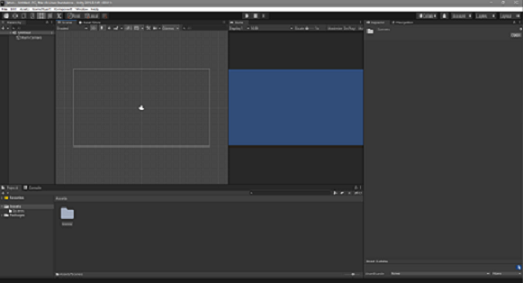
\includegraphics{img/Unity-Editor}
%	\caption{Unity-Editor}
%	\label{fig:Editor}
%\end{figure}

%% ==============================
\section{Unity}
%% ==============================
\label{ch:Implementierung:sec:Unity}

Die ersten Versuche einer lauffähigen Umsetzung habe ich mit einem vorgefertigten Spielbrett umgesetzt. Dabei habe ich das Brett durch 8x8 einzelne Zellen beziehungsweise Quadrate dargestellt. Auf diesen Quadraten habe ich die Spielsteine als schwarze und graue Kreise platziert und diesen via Skript Funktionen gegeben. Dieser erste Entwurf (Abbildung \ref{fig:Prototyp}) reagierte auf das OnClick()-Event, sodass beim Anklicken eines Kreises der mögliche Weg hervorgehoben wurde und beim Klick auf das gewünschte Feld, wurde der Kreis auf diesem neuen Feld platziert.
Da dieser Entwurf sehr statisch und die Größe fest verankert war, habe ich mir Informationen gesucht um das Spiel dynamisch zu erstellen und die Größe des Spielfelds variabel zu machen. Dazu habe ich sowohl für die Zellen, als auch die Spielsteine Prefabs erstellt und somit mittels Skript in der Start-Funktion die Prefabs abgerufen und je nach angegebener Größe das Spielfeld zur Laufzeit erstellt.
Außerdem wurde das OnClick()-Event durch Drag \& Drop ersetzt, sodass es auf einem Touchscreen intuitiver zu bedienen ist.
%% ==============================
\section{GameObjects}
%% ==============================
\label{ch:Implementierung:sec:GameObjects}
Um die einzelnen Spielelemente darzustellen, müssen im Unity-Editor erst Spielobjekte (englisch: GameObject) erstellt werden. Die folgenden Objekte wurden dem Spiel hinzugefügt:
\paragraph{Main Camera}
Die Kamera ist zuständig für das Sichtfeld, sodass hier festgelegt werden kann, was innerhalb der Szene sichtbar ist.
\paragraph{Board}
Das \textbf{Board} ist das Objekt, dass das Spielbrett darstellt. Via Prefabs werden dem Board zur Laufzeit die einzelnen Zellen hinzugefügt und so das Brett aufgebaut.
\paragraph{PieceManager}
Der \textbf{PieceManager} ist zuständig für die einzelnen Spielsteine, die ebenfalls via Skript und Prefab der Szene und dem PieceManager hinzugefügt werden.
\paragraph{GameManager}
Der \textbf{GameManager} beinhaltet die Spiellogik und lässt das Spiel starten, sowie auch beenden. Hier wird nach jedem Zug geprüft ob ein Spieler gewonnen hat oder das Spiel noch weiter läuft. Weiterhin wird hier die Berechnung der KI angestoßen.
\paragraph{EscapeMenuManager}
Der \textbf{EscapeMenuManager} ist zuständig für das Event-Handling des Menüs und der Buttons. Das heißt, hier wird entschieden, ob das Menü sichtbar und was in dem Menü zu sehen ist.

%% ==============================
\section{Skripte}
%% ==============================
\label{ch:Implementierung:sec:Skripte}
Damit die einzelnen Objekte auch Funktionen und Informationen bekommen, musste jedem Objekt ein Skript hinzugefügt werden.
Beispielsweise hat jeder Spielstein das Skript \textbf{SimplePiece} zugeordnet bekommen. Dieses ermöglicht dem Spielstein die Bewegungen auf dem Spielbrett durchzuführen. Es enthält Funktionen die auf das Ein- und Austreten des Drag\&Drop-Events reagieren. Des Weiteren werden hier Informationen über die Ursprungszelle, sowie die aktuelle Zelle gespeichert um das Zurücksetzen des Spiels für einen Neustart nach dem Beenden eines Spiels zu vereinfachen. \\
Das \textbf{PieceManager}-Skript ist für die Spielsteine insgesamt zuständig, das heißt hier werden die Prefabs und Skripte der Spielsteine instanziiert und der Szene hinzugefügt beziehungsweise auf dem Spielbrett platziert. Außerdem kann dieser Manager die Funktionen der Spielsteine ein und ausschalten, sodass nur mit den Steinen interagiert werden kann, die auch gerade am Zug sind, vorausgesetzt das Spiel befindet sich nicht im Simulations-Modus.\\
Der \textbf{EscapeMenuActivator} ist für das Ein- und Ausschalten des Menüs zuständig.\\
Der \textbf{GameManager} stößt jeden Spiel-relevanten Prozess an, speichert ob eine oder zwei KIs aktiviert sind und lenkt dementsprechend das Spielgeschehen. Das Spiel wird hier auch gestartet und beendet.\\
Das Spielbrett erhält das \textbf{Board}-Skript und initiiert den Aufbau des Spielbretts. Außerdem werden hier alle Zellen und deren Anordnung gespeichert, sodass das Board mögliche Züge validieren kann.\\
Für die Berechnungen der KI erbt das Skript \textbf{BoardDraught} die Funktionen und Variablen des Board-Skriptes, übernimmt aber nur die wichtigen Informationen.\\
Jede Zelle erhält ebenfalls ein eigenes Skript (\textbf{Cell}), dass die Position der Zelle beinhaltet und den Spielstein, der sich auf der Position befindet. Außerdem wird hier das Hervorheben der Zellen durchgeführt.\\
Die Klasse \textbf{Move} enthält Informationen für eine mögliche Bewegung, das heißt hier wird die aktuelle Position des gerade betrachteten Spielsteins gespeichert, sowie die Zelle auf welche sich der Stein bewegen kann. Weiterhin enthält diese verschiedene Flags, die zur Bewertung der Aktion dienen.\\
Im \textbf{AIManager} befindet sich der MiniMax-Algorithmus, der die Berechnungen und Bewertungen der möglichen Züge durchführt. Wie genau der Algorithmus funktioniert wird im nachfolgenden Abschnitt erklärt.

%% ==============================
\section{MiniMaxing}
%% ==============================
\label{ch:Implementierung:sec:MiniMaxing}
Für die Implementierung des MiniMax-Algorithmus habe ich die Klasse AIManager entworfen. Diese enthält die Funktion \textbf{Minimax()}, die sich an der beschriebenen Umsetzung von Jorge Palacios\cite{palacios2016unity} orientiert. Diese übernimmt das aktuelle Spielbrett als Board, die maximale Suchtiefe, die aktuelle Tiefe und den Spieler der am Zug ist. Die Berechnungen und Evaluation der möglichen Züge werden anschließend hier rekursiv durchgeführt und es wird die maximal erreichte Punktzahl zurückgegeben, sowie die Referenzierung des zugeordneten Zuges.\\
\begin{figure}[h]
\begin{lstlisting}[basicstyle=\scriptsize\ttfamily, numbers=left, stepnumber=1, numberstyle = \tiny]
public static float Minimax(BoardDraught board, int player, int maxDepth,
int currentDepth, ref Move bestMove)
{
	if (board.IsGameOver() || currentDepth == maxDepth)
		return 0;
	bestMove = null;
	float bestScore = Mathf.Infinity;
	if (board.GetCurrentPlayer() == player)
	bestScore = Mathf.NegativeInfinity;
	List<Move> allMoves = new List<Move>();
	int nextPlayer = 0;
	if (player == 2){
		allMoves = board.GetMoves(player);
		nextPlayer = 1;
	}
	else if (player == 1){
		allMoves = board.GetMoves(player);
		nextPlayer = 2;
	}
	Move currentMove;
	float score = 0;
	foreach (Move m in allMoves){
		board.MakeMove(m);
		float currentScore = 0;
		currentMove = m;
		if (m.attacked)	{
			if (nextPlayer == 2)
			nextPlayer = 1;
			else
			nextPlayer = 2;
		} 
		currentScore = Minimax(board, nextPlayer, maxDepth, 
				currentDepth + 1, ref currentMove);
		float newScore = board.Evaluate(player);
		if (board.GetCurrentPlayer() == player)	{
			currentScore += newScore;
			if (currentScore > bestScore)
			{
				bestScore = currentScore;
				bestMove = m;
				m.mScore = bestScore;
			}
		}
		else{
			currentScore -= newScore;
			if (currentScore < bestScore){
				bestScore = currentScore;
				bestMove = m;
				m.mScore = bestScore;
			}
		}
		board.StepBack();
		if (m.attacked){
			if (nextPlayer == 2)
				nextPlayer = 1;
			else
				nextPlayer = 2;
		} 
	}
	List<Move> bestMoves = new List<Move>();
	if (currentDepth == 0){
		foreach (Move m in allMoves){
			if (m.mScore == bestScore){
				bestMoves.Add(m);
			}
		}
		System.Random rnd = new System.Random();
		int index = rnd.Next(bestMoves.Count);
		bestMove = bestMoves.ToArray()[index];
	}
	return score;
}
\end{lstlisting}
\caption{MiniMax}
\label{fig:MiniMax}
\end{figure}
\paragraph{Funktionsaufruf MiniMax}
Die rekursive Funktion \textbf{Minimax()} wird aufgerufen und bekommt sowohl den momentanen Spielzustand, die maximale \& aktuelle Suchtiefe, als auch eine Referenzierung auf einen Zug, der nachher der beste zugeordnet wird, übergeben. Somit sind alle nötigen Informationen zur Berechnung vorhanden und es kann, wie in Abbildung~\ref{fig:MiniMax}
zu sehen ist, in Zeile 4 die Startbedingung geprüft werden. Falls das Spiel beendet ist oder die maximale Suchtiefe erreicht wurde, wird eine 0 zurückgegeben. Anschließend werden die möglichen Züge des gerade betrachteten Spielers innerhalb der \textbf{BoardDraught}-Klasse berechnet. Zeile 14 prüft, ob es sich um den ersten oder zweiten Spieler handelt, ruft dementsprechend die Züge des Spielers ab und speichert diese in der Variablen allMoves. In der ForEach-Schleife wird über die von diesem Zustand aus möglichen Züge iteriert. Dabei wird zuerst die Bewegung auf dem Spielbrett simuliert und auf diesem gespeichert, um nach jeder Iteration den Schritt rückgängig machen zu können. In Zeile 31 wird geprüft, ob der Spieler einen gegnerischen Stein erobern würde. Falls ein Angriff stattgefunden hat, wird der nächste Spieler auf den aktuellen Spieler gesetzt, sodass dieser in der darauffolgenden Suchtiefe wieder betrachtet wird. Zeile 38 startet die Rekursion mit dem neuen Spielzustand und speichert die Punktzahl in currentScore. Anschließend wird die aktuelle Bewegung evaluiert und die entsprechenden Punkte zurückgegeben und in newScore zwischengespeichert. Zum Schluss werden die Punkte aus newScore auf die aktuelle Punktzahl addiert, falls der betrachtete Spieler auch derjenige ist, der am Zug ist, oder subtrahiert, wenn der Gegenspieler dran wäre. Schließlich wird in Zeile 61 mit der Board-Funktion \textbf{StepBack()} der letzte Zug rückgängig gemacht und die Iteration wird fortgesetzt. Nach der Rekursion sollten alle Aktionen eine Bewertung erhalten haben. Da die Punktzahl teilweise identisch war, wurde immer der erste betrachtete Zug mit der maximal erreichten Punktzahl gewählt. Daher habe ich noch einen Zufallsgenerator implementiert, der eine zufällige Bewegung aus denen mit der höchsten und selben Punktzahl auswählt und zurückgibt.\\
\begin{figure}[h]
\begin{lstlisting}[basicstyle=\scriptsize\ttfamily, numbers=left, stepnumber=1, numberstyle = \tiny]
public float Evaluate(string color)
{
	float eval = 1f;
	int rows = sizeX;
	int cols = sizeY;
	if (currentMove.attacked)
		eval += pointAttacked;
	if (currentMove.attacked2)
		eval += pointAttacked;
	if (currentMove.threaten)
		eval += pointThreat;
	if (currentMove.highThreat)
		eval += pointHighThreat;
	if (currentMove.hide)
		eval += pointHide;
	if (IsGameOver())
		eval += pointSuccess;
	currentMove.mScore += eval;
	return eval;
}
\end{lstlisting}
\caption{Evaluierungs-Funktion Version 1}
\label{fig:eval1}
\end{figure}
\paragraph{Evaluierung}
Die \textbf{Evaluate()}-Funktionen sind für die Bewertung der Züge zuständig. Sobald die Funktion \textbf{Evaluate()} aus der Abbildung~\ref{fig:eval1} aufgerufen wird %Dabei ruft \textbf{Evaluate(int player)} die \textbf{Evaluate(string color)}-Funktion mit der zugeordneten Farbe für Entscheidungen in der Evaluierung auf.
 findet die eigentliche Punkteverteilung statt. Jeder Zug hat zuvor für verschiedene Spielsituationen Flags zugeordnet bekommen. Diese werden bei der Suche nach möglichen Bewegungen auf \textit{true} gesetzt, wenn die definierte Bedingung zutrifft. Beispielsweise wird das \textit{Attacked}-Flag gesetzt, wenn der Zug zu einer Eroberung führt und die Aktion erhält die vorher festgelegte Punktzahl für Angriffe. Das Flag \textit{attacked2} wird gesetzt, wenn zwei Steine in diesem Zug erobert werden können. \textit{Threaten} wird \textit{true}, wenn die Aktion zu einer Bedrohung für den Gegenspieler führt. \textit{HighThreat} wurde eingeführt um Bedrohungen, die im nächsten Zug zur Eroberung führen, besser bewerten zu können. Das \textit{Hide}-Flag steht für den Abzug aus einer eigenen Bedrohung, also werden hier Punkte für ein defensives Verhalten verteilt. Zum Schluss wird geprüft ob das Spiel nach dem Zug beendet wäre und dementsprechend die Punktzahl dazu addiert. Die Punkteverteilung bestimmt auch den Schwierigkeitsgrad. Nach dem Testen dieses Bewertungssystem hat sich herausgestellt, dass diese Bewertung noch zu unpräzise ist. Um die KI noch intelligenter zu machen, wurden weitere wichtige Spielsituationen betrachtet und die Evaluierung um Kriterien ergänzt.
\paragraph{Verbesserung der Evaluierungs-Funktion}
Die zuvor beschriebene Evaluierung wurde zu grob gestaltet, sodass wichtige Situationen nicht oder zu wenig betrachtet wurden. Dabei ist aufgefallen, dass die KI vor allem akute Bedrohungen der eigenen Steine nicht erkannt hat. Daher wurden die Flags ,,danger'', ,,squadHide'' \& ,,isSquadHide'', ,,prepSquadHide'' \& ,,isPrepSquad'', ,,corner'' \& ,,isInCorner'', ,,OOBAndFriendlyCorner'' \& ,,isOOBAndFriendlyCorner'' und ,,highAlert'' hinzugefügt wie in der Abbildung \ref{fig:eval2} zu sehen ist. Dabei steht ,,squadHide'' für eine Vierer-Formation auf dem Spielfeld (vgl. Abbildung \ref{fig:squad}), die vom Gegner nicht erobert werden kann. Diese Formation ist aufgrund der fehlenden Möglichkeit eingenommen werden zu können, die wichtigste Verteidigungsstellung im Spiel. ,,PrepSquadHide'' ist ein Flag, dass die Vorbereitung auf die Vierer-Stellung darstellt. Es steht also für eine L-Förmige Formation auf dem Spielfeld, wie die Steine es in \ref{fig:squad} abbilden. Das Flag ,,danger'' steht für eine akute Gefahr und wurde so implementiert, dass erkannt wird, wenn ein bedrohter Stein von einem weiteren gegnerischen erreichbar ist und beeinflusst die Puntkeverteilung insofern, dass bei aktivem Danger-Flag die Gewichtung der Verteidigungs-Flags des bedrohten Steins erhöht werden. ,,Corner'' steht für eine Eckposition aus der kein Stein erobert werden kann. ,,OOBAndFriendlyCorner'' ist der Indikator für eine Position am Rand des Spielbretts und neben einer Eckposition, die von einem eigenen Stein bereits belegt ist. Das Flag ,,highAlert'' wird gesetzt, wenn der betrachtete Stein erobert werden kann. Das Prefix ,,is'' steht für das jeweils äquivalente Flag des Ist-Zustands und beeinflusst die Gewichtung der Punkte. \\Darüber hinaus wurde noch die Suchtiefe in die Evaluierung aufgenommen. Dadurch wird durch steigende Suchtiefe die Gewichtung der Spielzustände reduziert. Als Beispiel betrachten wir die Suchtiefe 10. Der Zustand mit der Tiefe $1$ erhält eine Gewichtung von $1$. Wohingegen der Zustand der Tiefe 10 nur noch eine Gewichtung von $0.1$ erhält und so weniger Einfluss auf die Bewertung hat. Dadurch soll vermieden werden, dass die Punkteverteilung der Zustände unterschiedlicher Tiefe sich zu sehr ausgleichen. Außerdem wurde die Anzahl der verfügbaren Spielsteine in die Analyse aufgenommen. Die Punkteverteilung während dem Spiel wird dadurch beeinflusst. Die Idee dahinter ist es, dass die KI sich aggressiver verhält, wenn sie aktuell mehr Steine des Gegenspielers erobert hat. Außerdem soll sich die KI dadurch auch eher in Verteidigungspositionen begeben, falls der Gegenspieler mehr Spielsteine auf dem Feld hat.
\begin{figure}
	\centering
	\includegraphics{img/Squad2}
	\caption{Vierer-Formation und L-Form}
	\label{fig:squad}
\end{figure}
\begin{figure}[h]
	\begin{lstlisting}[basicstyle=\scriptsize\ttfamily, numbers=left, stepnumber=1, numberstyle = \tiny]
public float Evaluate(string color)
{
	dangerMultiplier = 1f;
	attackWeight = 1f;
	if (danger)
	{
		dangerMultiplier = 2f;
	}
	if (isInCorner)
	{
		eval += -20;
	}
	if (isPrepSquad)
	{
		eval += -10;
	}
	if (isInCorner && attacked && !highAlert)
	{
		attackWeight = 3f;
	}
	if (isOOBAndFriendlyCorner)
	{
		eval += -50;
	}
	else if ((isOOBAndFriendlyCorner || isSquadHide) && threaten && !attacked)
	{
		attackWeight = 2f;
	}
	else if ((isOOBAndFriendlyCorner || isSquadHide) && threaten && !attacked)
	{
		attackWeight = 1.25f;
	}
	else if (isOOBAndFriendlyCorner && attacked && !highAlert)
	{
		attackWeight = 3f;
	}
	else if (isOOBAndFriendlyCorner && attacked && highAlert)
	{
		attackWeight = 3f;
	}
	else if (attacked)
	{
		attackWeight = 2f;
	}
	if (attacked)
		eval += pointAttacked * attackWeight;
	if (attacked2)
		eval += pointAttacked * attackWeight;
	if (attacked2)
		eval += pointAttacked * attackWeight;
	if (threaten)
		eval += pointThreat * attackWeight; ;
	if (hide)
		eval += pointHide * dangerMultiplier;
	if (squadHide)
		eval += pointSquadHide * dangerMultiplier;
	if (prepSquad)
		eval += pointPrepSquad * dangerMultiplier;
	if (corner)
		eval += pointCorner * dangerMultiplier;
	if (OOBAndFriendlyCorner)
		eval += pointOOBAndCorner*dangerMultiplier;
	if (highAlert)
		eval += pointHighAlert;
	if (highThreat)
		eval += pointHighThreat;
	if (IsGameOver())
		eval += pointSuccess;
	return eval;
	}
	\end{lstlisting}
	\caption{Evaluierungs-Funktion Version 2}
	\label{fig:eval2}
\end{figure}
\paragraph{Analyse der Ausgangssituation}
Das System wurde um eine Analyse der Ausgangssituation erweitert um Bedrohungen besser ausweichen zu können oder wichtige Positionen nicht zu verlassen. Hier wird geprüft ob der aktuelle Stein in Gefahr ist und dementsprechend die Gewichtung dieser Züge erhöht, um aus der Situation fliehen zu können. Des weiteren werden unschlagbare Positionen höher gewichtet. Befindet sich ein Stein in der Ecke des Spielfelds, wird die Gewichtung der Verteidigungs-Flags erhöht, sodass die Stellung nur für Eroberungen oder sichere Bedrohungen des Gegners verlassen wird. Eine sichere Bedrohung ist so definiert, dass ein Stein sich neben dem Gegenspieler positionieren kann ohne im nächsten Zug geschlagen werden zu können. Außerdem wurde das Flag ,,isInCorner'' eingeführt, welches evaluiert, ob der Spielstein sich in einer Ecke befindet. Dann wird der Gesamtpunktzahl ein Wert $x$ abgezogen um die Stellung nicht zu verlassen, außer es sind keine anderen Züge möglich oder es kann eine Spielfigur eingenommen werden. Außerdem wird in der Abbildung \ref{fig:eval2} Zeile 21 geprüft, ob der Stein sich am Rande des Spielfelds und neben einem weiteren eigenen befindet, da dies ebenfalls eine unschlagbare Position bildet.


% könnte die Evaluierung noch um eine beliebige Anzahl an Flags erweitert werden, sodass die Spielsituation immer präziser bewertet wird.

%%% Local Variables: 
%%% mode: latex
%%% TeX-master: "thesis"
%%% End: 
    % Implementierung
%% eval.tex
%% $Id: eval.tex 61 2012-05-03 13:58:03Z bless $

\chapter{Evaluation}
\label{ch:Evaluierung}
%% ==============================
%Hier erfolgt der Nachweis, dass das in Kapitel~\ref{ch:Entwurf}
%entworfene Konzept funktioniert. 
%Leistungsmessungen einer Implementierung werden immer gerne gesehen.
Zur Evaluation wurde eine lauffähige Windows Version und Webversion dem Landesmuseum Birkenfeld zugesendet. Außerdem wurde das Verhalten der KI mit unterschiedlichen Konfigurationen gegen einen menschlichen Spieler, sowie als Simulation analysiert.

%% ==============================
\section{Launch beim Kunden}
%% ==============================
\label{ch:Evaluierung:sec:Launch}
Die erste spielbare Version mit den grundlegenden und erweiterten Features wurde dem Landesmuseum mittels GitHub und E-Mail zugesendet, sodass diese Version trotz anhaltender Kontaktbeschränkungen vor Ort getestet werden konnte. Herr Decker hat uns während einem GoToMeeting-Videoanruf die Testversion auf ihrem Gerät zeigen können. Dabei wurde klar, dass die grundlegenden und erweiterten Features funktionieren. Es wurde festgestellt, dass erfahrene Spieler der implementierten KI überlegen sind und regelmäßig gewinnen. Das Spiel gegen die KI wurde zuvor von Personen, die sich nicht mit Latrunculi auseinandergesetzt haben, getestet und verloren, allerdings auch nicht in jeder Runde. Das Hervorheben der erlaubten Positionen wurde auf dem vorhandenen Gerät nicht wieder entfernt, wenn der Spieler seine Züge zu schnell erledigt hat. Außerdem sind die Spielsteine teilweise zwischen den Zellen hängen geblieben und nicht auf der korrekten Position eingerastet. Diese beiden Punkte waren auf meinen Testgeräten nicht reproduzierbar, daher liegt die Vermutung nahe, dass es ein hardwarespezifisches Problem des genutzten Touch-Tisches vor Ort im Museum ist. Aufgrund der Kontaktbeschränkungen ist es aktuell auch nicht möglich, die Version persönlich vor Ort zu testen, um Fehlerquellen einzugrenzen. Ein weiterer auffälliger Punkt war, dass das Menü auf dem Gerät vor Ort zu klein wirkte und sich nicht an die Bildschirmgröße angepasst hat. Meine Geräte haben maximal eine Größe von 22 Zoll, sodass es zuvor nicht möglich war, es auf einem vergleichbaren Gerät mit einer Größe von 55 Zoll zu testen.
Ein weiterer Punkt, der sich gewünscht wurde, war, dass die KI deaktivierbar sein soll, damit das Spielen zwischen zwei Personen möglich ist.

%% ==============================
\section{Verhalten in der Simulation ohne Analyse der Ausgangssituation}
%% ==============================
\label{ch:Evaluierung:sec:Simulation}
Zur Analyse des Simulationsverhalten wurden verschiedene Konfigurationen ausprobiert und beobachtet. Die erste Einstellung hat eine Suchtiefe von 3 und folgende Punkteverteilung: \\
\paragraph{Spieler 1 (Muscheln):}
\begin{itemize}
	\item Angriffspunkte: 80
	\item Verteidigungspunkte: 50
	\item Bedrohungspunkte: 20
	\item Hohe Bedrohungspunkte: 0
\end{itemize}

\paragraph{Spieler 2 (Steine):}
\begin{itemize}
	\item Angriffspunkte: 100
	\item Verteidigungspunkte: 20
	\item Bedrohungspunkte: 50
	\item Hohe Bedrohungspunkte: 80
\end{itemize}
Beide KIs wirken mit diesen Einstellungen sehr aggressiv. Der erste Zug eines Spiels, ist einer auf ein Feld ohne Feindkontakt. Anschließend bedroht der zweite Spieler die bewegte Figur, indem der Spielstein sich unmittelbar daneben platziert. Im nächsten Zug wird der zuletzt bewegte Stein erobert. Insgesamt wirkt die KI auf beiden Seiten als würde sie möglichst viele gegnerische Figuren bedrohen und angreifen wollen, auch wenn es eine eigene Bedrohung zur Folge hat. Außerdem fällt auf, dass die Muscheln mehr Eroberungen erreichen. Hier lässt sich festhalten, dass in 7 von 10 Spielrunden die Muscheln gewonnen haben. Allerdings wird erkennbar, dass die Steine durch das zusätzliche Flag Bedrohungen der Muscheln einleiten, die dadurch theoretisch im nächsten Zug erobert werden könnten.
\paragraph{Suchtiefe: 10}
Bei selber Konfiguration wie zuvor, aber erhöhter Suchtiefe, fällt auf, dass die Steine  auch versuchen Muscheln zu bedrohen, die nicht in einem Zug erreichbar sind. Dieses Verhalten führt allerdings auch dazu, dass die Muscheln diesen zusätzlichen Zug teilweise ausnutzen, um die bewegte Figur zu erobern. Die Gewinnchance bei 10 gespielten Runden ist gleich verteilt, sodass beide jeweils 5 gewonnen haben. Aufgefallen ist dabei, dass es gegen Ende des Spiels zu Situationen kommen kann, in denen beide Spieler ihre verbliebenen Steine (hier waren es jeweils zwei) immer wieder hin und her bewegen, ohne dabei zu einem Angriff zu kommen. Die KIs bewerten die Bedrohungen in so einer Situation so hoch, dass sie sich dadurch zuerst scheinbar ,,festfahren''.
\paragraph{Erhöhte Verteidigungspunkte und verminderte Angriffspunkte mit Suchtiefe 3}
\paragraph{Spieler 1 (Muscheln):}
\begin{itemize}
	\item Angriffspunkte: 80
	\item Verteidigungspunkte: 50
	\item Bedrohungspunkte: 20
	\item Hohe Bedrohungspunkte: 70
\end{itemize}
\paragraph{Spieler 2 (Steine):}
\begin{itemize}
	\item Angriffspunkte: 20
	\item Verteidigungspunkte: 100
	\item Bedrohungspunkte: 50
	\item Hohe Bedrohungspunkte: 80
\end{itemize}
Für die folgende Beobachtung wurden die Verteidigungspunkte der Steine mit den Angriffspunkten der ersten Konfiguration vertauscht und den Muscheln wurde ebenfalls das Flag der Hohen Bedrohung mitgegeben. Die beobachteten 10 Runden endeten jedes mal mit einem Sieg der Muscheln. Dabei ist aufgefallen, dass das Verteidigungs-Flag Wirkung zeigt und die Steine sich aus Bedrohungen zurückziehen. Allerdings führt das weniger aggressive Verhalten dazu, dass die Steine im Endeffekt die Runden verlieren. Außerdem gab es die Situation aus Abbildung \ref{fig:nicht erkannt}, in der die Muscheln nicht erkannt haben, dass die Steine eingekesselt werden können und somit das Spiel gewonnen wäre. Die Spieler haben ihre Spielsteine so lange bewegt, bis es für die Muscheln möglich war, einen zu erobern und dadurch das Spiel zu gewinnen.
\begin{figure}[h]
	\centering
	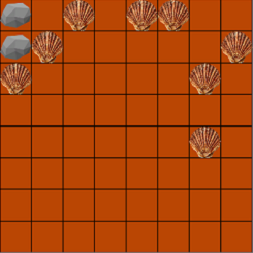
\includegraphics{img/einkesselnHidezuhoch2}
	\caption{Spielende wird nicht erkannt}
	\label{fig:nicht erkannt}
\end{figure}
\paragraph{Suchtiefe 10}
Bei erhöhter Suchtiefe haben die Steine 4 von 10 Runden gewonnen. Hier ist aufgefallen, dass mehr Angriffe über 2 Züge stattfinden. Dieses Verhalten kann auf die erhöhte Suchtiefe zurückgeführt werden. Dadurch können zukünftige Züge evaluiert werden und so Eroberungen die in späteren Zügen erst möglich sind durchgeführt werden. Insgesamt erweckt die KI allerdings den Eindruck, dass sie möglichst oft versucht gegnerische Spielsteine zu erobern. Aufgrund des zu aggressiven Verhaltens wurde die Analyse der Ausgangssituation implementiert, sowie weitere Flags für eine präzisere Bewertung.

%% ==============================
\section{Verhalten der KI ohne Analyse der Ausgangssituation gegen einen menschlichen Spieler}
%% ==============================
\label{ch:Evaluierung:sec:KIvsHuman}
\paragraph{Spieler 2 (Steine):}
\begin{itemize}
	\item Angriffspunkte: 100
	\item Verteidigungspunkte: 20
	\item Bedrohungspunkte: 50
	\item Hohe Bedrohungspunkte: 80
	\item Suchtiefe: 3
\end{itemize}
Die KI hat mit diesen Konfigurationen eine sehr aggressive Spielweise gezeigt. Dabei ist aufgefallen, dass vor allem die Bedrohung und Angriffe im Fokus stehen. Mit dieser Konfiguration war es möglich den Computer mit simplen Spielzügen aus der Verteidigung zu locken und die Steine zu erobern. Es wurden regelmäßig Steine neben Muscheln platziert, auch wenn es im nächsten Zug eine eigene Eroberung zur Folge hat. Der Verteidigungsmechanismus kommt in dieser Konfiguration nur selten zur Geltung. Einerseits sind dazu die defensiven Punkte zu gering angesetzt, sodass diese kaum Auswirkungen auf die Spielzüge haben. Andererseits wurde hier auch eine geringe Suchtiefe gewählt, sodass die Verteidigung noch weniger ins Gewicht fällt und somit kaum Relevanz im Spiel zeigt. Um zu sehen, ob sich das Verhalten ändert, wurde die Suchtiefe auf 10 erhöht.

\paragraph{Spieler 2 (Steine):}
\begin{itemize}
	\item Angriffspunkte: 100
	\item Verteidigungspunkte: 20
	\item Bedrohungspunkte: 50
	\item Hohe Bedrohungspunkte: 80
	\item Suchtiefe: 10
\end{itemize}

Mit dieser Konfiguration wirkte die KI noch immer sehr aggressiv und hat kaum eine Möglichkeit ausgelassen, die Muscheln anzugreifen. Diese wurden in der Regel schnell wahrgenommen und umgesetzt, sodass allerdings im nächsten Zug wieder der angreifende Stein erobert werden konnte. Allerdings führten ein paar Bedrohungen dazu, dass die KI sich zurückgezogen und neben einem eigenen Stein eingereiht hat und nun nicht mehr so einfach einzunehmen war. Insgesamt wurde das Spielverhalten nach wenigen Runden vorhersehbar und konnte leicht überlistet werden.

\paragraph{Spieler 2 (Steine):}
\begin{itemize}
	\item Angriffspunkte: 80
	\item Verteidigungspunkte: 70
	\item Bedrohungspunkte: 50
	\item Hohe Bedrohungspunkte: 60
	\item Suchtiefe: 3
\end{itemize}
Für diese weiteren Tests wurden die Punktzahlen angepasst. Dabei wurde die Angriffs- und Bedrohungspunkte etwas reduziert und die Verteidigungspunkte erhöht, um dem defensiven Verhalten eine höhere Gewichtung zu geben. Diese Punkteverteilung machte sich auch im Verhalten bemerkbar. Die KI hat nicht mehr auf jede bewegte Muschel reagiert und sich so auch in der Verteidigung gehalten, allerdings wird schnell klar, dass dieses Verhalten zu passiv war und die Steine schnell eingekesselt werden konnten, sodass kein weiterer Zug mehr möglich war. Die KI hat eigene Bedrohungen noch immer nicht erkennen können, hat dafür aber nicht mehr auf jede Möglichkeit sich den Muscheln zu nähern reagiert. Anschließend wurde wieder die selbe Konfiguration mit der Suchtiefe 10 betrachtet.

\paragraph{Spieler 2 (Steine):}
\begin{itemize}
	\item Angriffspunkte: 80
	\item Verteidigungspunkte: 70
	\item Bedrohungspunkte: 50
	\item Hohe Bedrohungspunkte: 60
	\item Suchtiefe: 10
\end{itemize}
Mit dieser Veränderung hat die KI es geschafft, weniger durchdachte Züge zum eigenen Vorteil zu nutzen und Muscheln zu erobern. Allerdings passierte dies auf Kosten der eigenen Steine. Die KI wirkt insgesamt noch immer aggressiv und verliert in der Regel gegen geübte Spieler. Insgesamt hat sich gezeigt, dass die entwickelte KI noch zu primitiv ist und eigene Bedrohungen nicht zu erkennen scheint.\\
Daher wurden für weitere Analysen zusätzliche Kriterien implementiert, die unter anderem auch die aktuelle Spielsituation besser beschreiben und eigene Bedrohungen erkennen lassen. Das heißt, es wurde die Möglichkeit implementiert zu erkennen, dass ein Angriff zu eigenen Bedrohungen führen kann. Weiterhin wurden Situationen integriert, die dafür sorgen sollen, dass die Steine sich auch in Vierer-Formationen platzieren können. Diese Zählen zu den stärksten Zügen in diesem Spiel, da es schlicht nicht möglich ist Spielsteine aus dieser Formation zu erobern. Weiterhin wurden Positionen am Rand des Spielbretts und vor allem die Ecken höher priorisiert. Um das ganze System von der Situation abhängig machen zu können, wurden Multiplikatoren als Gewichtung eingesetzt, die während der Evaluierung variieren können.
%% ==============================
\section{Verhalten in der Simulation mit Analyse der Ausgangssituation}
%% ==============================
\label{ch:Evaluierung:sec:SimulationWithAnalyse}
Für die folgenden Beobachtungen wurde die Simulation mit zusätzlichen gewichteten Analysekriterien betrachtet. Dabei gelten bei den ersten Tests die gleichen Punkteverteilungen für beide KIs und eine Suchtiefe von 10.\\
Dies spiegelt sich stark in ihrem Verhalten wieder. Sowohl die Steine, als auch die Muscheln finden sehr schnell die wichtigen Positionen um nicht geschlagen zu werden. Haben beide Ihre unschlagbaren Positionen gefunden, dann bewegen sie sich nur noch zwischen den Verteidigungspositionen hin und her wie in Abbildung \ref{fig:hinundher} zu sehen ist. Dieses Verhalten hat sich endlos wiederholt.
\begin{figure}[h]
	\centering
	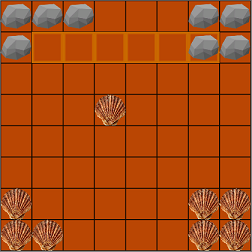
\includegraphics{img/mitAnalyse/hinundherCorner}
		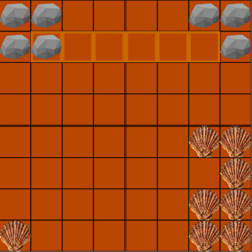
\includegraphics{img/mitAnalyse/hinundherCorner3}
	\caption{Steine und Muscheln mit der gleichen defensiven Konfiguration:\newline Links mit Suchtiefe 10 und rechts mit Suchtiefe 3}
	\label{fig:hinundher}
\end{figure}

Zum Vergleich wurde diese Konfiguration mit angepasster Suchtiefe auf 3 übernommen und ebenfalls als Simulation getestet. Aufgefallen ist, dass beide KIs ein paar Züge mehr benötigen, um diese Eck-Positionen, wie in Abbildung \ref{fig:hinundher} zu sehen, zu finden und sich dort zu positionieren. Hier hat sich ebenfalls herausgestellt, dass diese Reduzierung nur dazu führt, die wichtigen Positionen später zu finden. Das Verhalten hat sich abgesehen von der längeren Suche nicht verändert.
Daran wird deutlich, dass es nicht sinnvoll ist die KIs mit gleicher defensiver Konfiguration als Simulation laufen zu lassen. Hier kann man sich zwar wichtige Positionen verdeutlichen, allerdings nichts darüber hinaus, da das Spiel so auch nicht enden wird. Für den folgenden Testlauf wurden die Punkte für die Angriffs-Flags erhöht und beobachtet.
\paragraph{Erhöhte Angriffs- und verminderte Verteidigungspunkte mit Suchtiefe 10}
Bei einer Suchtiefe von 10 fällt auf, dass die Muscheln zu Beginn sich eher in die Mitte des Felds bewegen, die Steine sich aber recht zügig in die Eckpositionen begeben. Dabei bilden erstere Reihenformationen, die eine wichtige strategische Formation im Spiel bilden, da die Steine nur noch von 2, statt von 4 Seiten angegriffen werden können. Die Simulation endet hier mit weniger aktiven Spielsteinen als im Test zuvor, allerdings fahren sich beide Spieler zum Ende hin wieder in den Eckpositionen fest.
\begin{figure}[h]
	\centering
	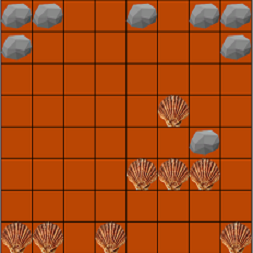
\includegraphics{img/reihe22}
	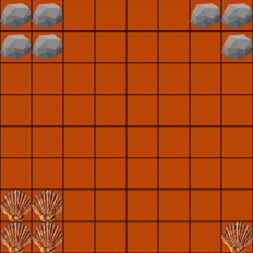
\includegraphics{img/Aggro/aggroEnde22}
	\caption{Steine und Muscheln mit der gleichen aggressiven Konfiguration und Suchtiefe 10: Links: Reihenformation \& rechts: Endsituation.}
	\label{fig:aggro}
\end{figure}
\paragraph{Erhöhte Angriffs- und verminderte Verteidigungspunkte mit Suchtiefe 3}
Bei diesen Einstellungen merkt man schnell, dass es länger dauert die Superpositionen zu finden. Die Spielsteine bewegen sich zuerst in die Mitte des Feldes, finden allerdings noch ihre verbündeten Steine, sodass sie sich nicht alleine offen ins Feld begeben. Allerdings tendieren sie nach wenigen Zügen dazu, sich wieder in die Ecken zu bewegen. Dabei stechen immer mal wieder Angriffe oder zumindest Angriffsversuche heraus. Zum Simulationsende hin fällt auf, dass immer wieder Versuche zur Bedrohung stattfinden, allerdings werden diese im darauffolgenden Zug wieder durch einen Rückzug hinfällig und die KIs befinden sich in einer Endlosschleife aus Bedrohung \& Rückzug, wie es in der Abbildung \ref{fig:aggro3} zu sehen ist.
\begin{figure}[h]
	\centering
	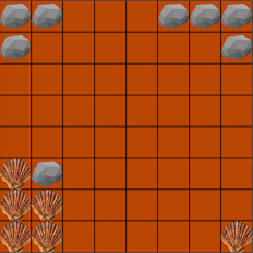
\includegraphics{img/Aggro/tiefe3Bedrohung2}
	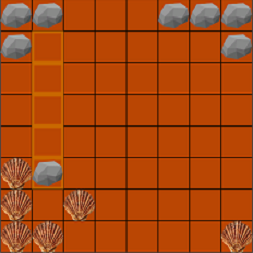
\includegraphics{img/Aggro/tiefe3rueckzug2}
	\caption{Steine und Muscheln mit der gleichen aggressiven Konfiguration und Suchtiefe 3: Endsituation.}
	\label{fig:aggro3}
\end{figure}

\paragraph{Flags mit gleicher Punkteverteilung und Suchtiefe 10}
Bei diesem Versuch wurden die verschiedenen Flags mit der gleichen Punktzahl belegt. Dabei ist aufgefallen, dass das Spiel insgesamt weniger intelligent verläuft und die Spielsteine sich teilweise in bedrohliche Positionen begeben. Gute Positionen werden noch immer erkannt, allerdings scheinen die KIs direkte Bedrohungen immer identifizieren zu können. Vorteilhaft an dieser Konfiguration ist, dass es bei Vorführungszwecken unwahrscheinlicher wird, dass die Simulation sich in einer Situation festfährt und keiner der beiden gewinnt. Insgesamt erkennt man trotzdem noch, dass Positionen neben verbündeten Steinen eher aufgesucht werden als offene mitten im Spielfeld. Teilweise stellt die KI sich neben gegnerische Steine, wird aber im darauffolgenden Zug erobert. 

\paragraph{Flags mit gleicher Punkteverteilung und Suchtiefe 3}
Mit verminderter Suchtiefe wirkt das Spielgeschehen noch zufälliger. Gute Positionen wie die Eckpunkte werden erkannt, genauso wie Positionen am Rand des Spielfelds und neben verbündeten Steinen. Allerdings fällt hier wieder auf, dass akute Bedrohungen nur noch teilweise erkannt werden. Wie zuvor mit der Suchtiefe 10 begeben sich die Steine in eine Bedrohungsposition, auch wenn im nächsten gegnerischen Zug die Steine erobert werden können. Stellenweise wirkt es, als würden Spielsteine des Gegners auf der eigenen Seite nicht erkannt werden. Hier bewegen sich die Steine ein paar Runden lang hin und her, wie in Abbildung \ref{fig:hinundherboth} bis die Muschel erobert wird.
\begin{figure}[h]
	\centering
	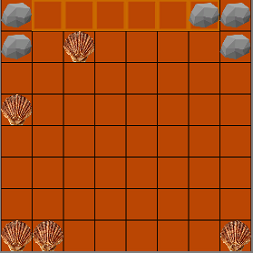
\includegraphics{img/both/muschelnichterkannt}

	\caption{Steine und Muscheln mit der gleichen Konfiguration und Suchtiefe erkennen mögliche Eroberung spät.}
	\label{fig:hinundherboth}
\end{figure}


\paragraph{Aggressive gegen Defensive KI}
Lässt man die aggressive gegen die defensive Konfiguration spielen, werden die Spielmechaniken deutlicher. Die defensive KI wirkt insgesamt stärker und sucht sich schnell gute Spielpositionen in den eigenen Ecken. Die aggressive versucht vor allem zu Beginn noch oft Steine zu erobern, verliert bei dem Versuch aber oft eigene. Allerdings orientiert sich diese auch mit steigender Rundenzahl in die Ecken und an den eigenen Steinen. Zur Vorführung scheint diese Einstellung am sinnvollsten, da Spielmechaniken wie Eroberungen und Verteidigungen klar werden. 
%% ==============================
\section{Verhalten der KI mit Analyse der Ausgangssituation gegen einen menschlichen Spieler}
%% ==============================
\label{ch:Evaluierung:sec:KIvsHumanWithAnalyse}
Die nachfolgenden Beobachtungen wurden bei einer Suchtiefe von 10 gemacht. Bei erhöhten Verteidigungspunkten und der Analyse des aktuellen Spielzustands hat das Spiel im Vergleich zu den Tests ohne Betrachtung der gegenwärtigen Situation bereits an Schwierigkeit gewonnen . Die KI macht einen intelligenteren Eindruck und lässt sich nicht mehr bei jeder Gelegenheit erobern. Weiterhin fällt hier auf, dass der Computer sich nach Angriffen auch wieder in eine sichere Position zurückzieht. Außerdem lassen die Steine sich auch nicht mehr aus ihrer Deckung locken, indem man die Muscheln einfach auf den mittleren horizontalen Reihen des Spielfelds zieht.\\
Betrachtet man die Konfiguration mit verminderter Verteidigungs- und erhöhter Angriffsgewichtung, scheint das Spielen gegen die KI schwerer zu werden. Die Steine ziehen sich immer wieder in die Eckpositionen zurück und versuchen in den meisten Fällen nur anzugreifen, wenn der Angriff nach Berechnung auch sicher ist. Diese Konfiguration wirkt sinnvoller als in der Simulation mit gleichen Einstellungen. Das Verhalten lässt sich so erklären, dass bei gleicher Punkteverteilung beide KIs versuchen ihre Spielsteine zu schützen und es nur selten zu Bedrohungen oder Angriffen kommt. Die KIs ziehen sich zurück, sobald erkannt wird, dass ein Angriff auf den Stein möglich ist. Da menschliche Spieler dazu tendieren können, die gegnerischen Spielsteine zu erobern, kommt der Verteidigungsmechanismus des Computers mehr zur Geltung.

\paragraph{Erhöhte Angriffs- und verminderte Verteidigungspunkte mit Suchtiefe 10}
Die KI hat sich mit diesen Einstellungen einkesseln lassen und so das Spiel schnell verloren. Insgesamt fällt auf, dass weniger defensiv gespielt wird als zuvor. Sie bewegt sich die meiste Zeit auf der eigenen Startseite, nutzt aber die Position clever aus, wenn sich ein Stein auf die gegnerische Spielseite bewegt hat. Die erhöhte Gewichtung der Angriffspunkte führt stellenweise zu Zügen in denen bis zu 3 Steine von mir erobert wurden.
\paragraph{Erhöhte Angriffs- und verminderte Verteidigungspunkte mit Suchtiefe 3}
Bei geringerer Suchtiefe hat sich die KI durch ein aggressives Verhalten schnell besiegen lassen. Bedrohungen wurden zwar erkannt, allerdings hat der Computer vor allem mit vielen Spielsteinen auf dem Feld sich seltener dafür entschieden, eine Bedrohung nicht einzugehen, wenn im nachfolgenden Zug der bewegte Stein erobert werden kann. Dieses Verhalten lässt sich auf die geringe Suchtiefe zurückführen. Gegen Ende des Spiels ist die Situation aus der Abbildung \ref{fig:nichtschlagbar} aufgefallen. Die KI hat sich nur noch in den Eckpositionen bewegt und hat sich nicht mehr in eine Situation bringen lassen, in der ich einen Stein erobern konnte.
\begin{figure}[h]
	\centering
	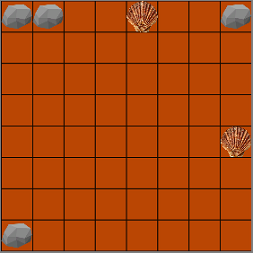
\includegraphics{img/Aggro/humannichtzuschlagen2}	
	\caption{Hohe Angriffspunkte bei Suchtiefe 3. KI weicht in die Ecken aus.}
	\label{fig:nichtschlagbar}
\end{figure}
\paragraph{Ausgeglichene Punkteverteilung}
Diese Einstellungen werden hauptsächlich durch die Gewichtung via Multiplikatoren beeinflusst. Das fällt auch im Spiel auf. Die Züge wirken teilweise nicht zielführend, wie zum Beispiel, wenn man sich neben einen computer-gesteuerten Stein platziert, entscheidet sich die KI stellenweise dafür diesen Stein durch eine Eroberung zu verlieren und bringt ihn nicht in Sicherheit. In der Abbildung \ref{fig:humaneingekesselt} erkennt man ein großes Problem bei diesen Einstellungen. Die KI hat sich zu Beginn des Spiels auf der eigenen Spielseite einkesseln lassen, sodass es nach nur einer Eroberung beendet war. Diese Situation entsteht dadurch, dass die KI sich mit ihrem ersten bewegten Stein nur eine Position nach vorne bewegt. Anschließend wird der Stein nur noch horizontal von einer Ecke zur nächsten geschoben. Diese Konfiguration ist bis hierhin die am wenigsten zielführende. Mit geringerer Suchtiefe lässt die KI sich ebenfalls wie in der Abbildung \ref{fig:humaneingekesselt} einkesseln und verliert dadurch das Spiel. Insgesamt wirkt diese Konfiguration sehr zurückhaltend, da die KI kaum versucht gegnerische Steine zu erobern.
\begin{figure}[h]
	\centering
	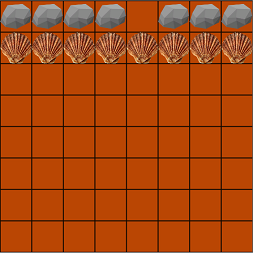
\includegraphics{img/both/humaneingekesselt}	
	\caption{KI lässt sich einfach einkesseln.}
	\label{fig:humaneingekesselt}
\end{figure}
%\paragraph{Flags mit gleicher Punkteverteilung und Suchtiefe 3}


%Bei erhöhter Suchtiefe 
%% ==============================
%\section{Zusammenfassung}
%% ==============================
%\label{ch:Evaluierung:sec:zusammenfassung}

%Am Ende sollten ggf. die wichtigsten Ergebnisse nochmal in \emph{einem} kurzen Absatz zusammengefasst werden.

%%% Local Variables: 
%%% mode: latex
%%% TeX-master: "thesis"
%%% End: 
        % Evaluation
%% entwurf.tex
%% $Id: entwurf.tex 61 2012-05-03 13:58:03Z bless $
%%

%\chapter{Mögliche Erweiterungen}
%\label{ch:Erweiterungen}
%% ==============================
%In diesem Kapitel erfolgt die ausführliche Beschreibung des eigenen
%Lösungsansatzes. Dabei sollten Lösungsalternativen diskutiert und
%Entwurfsentscheidungen dargelegt werden.


%% ==============================
\chapter{Alpha-Beta-Algorithmus}
%% ==============================
\label{ch:Erweiterung:sec:1.AB-Algo}
Um den Algorithmus effizienter zu gestalten, gibt es unterschiedliche Verfahren. Der Alpha-Beta-Algorithmus ist eine Möglichkeit eine geringere Laufzeit zu erzielen, indem frühzeitig Suchen abgebrochen werden, sobald absehbar ist, dass es eine bessere Alternative gibt.\nocite{AlphaBeta} Außerdem kann eine Verbesserung im Spielverhalten erzielt werden, wenn man mehr Bewertungskriterien einführt und so die Zustände präziser einordnen kann.
\nocite{edwards1961alpha} \\
Der Alpha-Beta-Algorithmus ist eine Verbesserung des MiniMax-Suchverfahrens. Dabei funktionieren beide prinzipiell ähnlich, allerdings werden durch ersteren im besten Fall die betrachteten Knoten von $2N$ auf $2N^{1/2}$ reduziert und soll so schneller in der Suche sein, wie es Griffith erläutert hat\cite{DBLP:journals/tc/Griffith76}.\\
Dabei entspricht Alpha dem besten bereits gefundenen Zug des maximierenden Spielers. Beta dem besten bisher gefundenen Zuges des minimierenden Spielers. Im Beispiel der Abbildungen \ref{fig:ab1} bis \ref{fig:ab8} kann das Prinzip leicht verständlich gemacht werden. Dabei entspricht der Spieler mit den Steinen dem maximierenden Spieler und der andere dem minimierenden. Alpha wird zu Beginn mit -$\infty$ und Beta mit $\infty$  festgelegt. Abbildung \ref{fig:ab1} zeigt den ersten Schritt. Dabei wird der linke Teilbaum zuerst durchsucht. Der betrachtete Spielzug des minimierenden Spielers hat eine Wertung von -30, deshalb wird in Abbildung \ref{fig:ab2} Beta mit -30 belegt. Nun wird das nächste Kind mit der Wertung -40 betrachtet und mit $\beta$ verglichen. -40 ist kleiner als -30, deshalb erhält $\beta$ in Abbildung \ref{fig:ab3} den kleineren Wert. Dies entspricht dem kleinsten erreichbaren Wert in dieser Situation und wird deshalb den Pfad entlang weitergereicht. In Abbildung \ref{fig:ab4} wird $\alpha$ dementsprechend mit -40 als Höchstpunktzahl des maximierenden Spielers gespeichert. Auf dem nächsten Ausschnitt \ref{fig:ab5} sieht man, dass $\alpha$ mit -40 als Vergleichswert gesetzt und $\beta$ wieder mit $\infty$ weitergereicht wird. Der Zug des maximierenden Spielers hat eine Punktzahl von +30 erhalten und der betrachtete Folgezug des Gegenspielers eine -40, daraus ergibt sich für $\beta$ -10. Wird der nächste mögliche Zug betrachtet, erreicht der minimierende Spieler eine -100 und wir erhalten ein $\beta$ von -70. Da -70 kleiner als $\alpha$ ist, kann, wie in Abbildung \ref{fig:ab7} zu sehen ist, der restliche Teilbaum gestrichen werden. Der Algorithmus geht immer von den bestmöglichen Zügen aus, daher ist es nicht mehr nötig die weiteren Zustände aus diesem Teilbaum zu betrachten. Die letzte Abbildung \ref{fig:ab8} zeigt die Betrachtung des dritten Baums. Hier erreicht $\beta$ wieder den Wert -70, sodass hier ebenfalls frühzeitig abgebrochen werden kann und wir erhalten -40 als maximale Punktzahl.
Das Abbrechen der Suche führt zu der vorher erwähnten Verkürzung der Laufzeit.


 %Die Durchsuchung des linken Teilbaums liefert eine -40 und wird als untere Schranke festgelegt. Als nächstes wird der mittlere Baum betrachtet. Hier erreicht der minimierende Spieler den Wert -100 im besten Fall und der maximierende erzielt +30 das in der Summe -70 ergibt. Also wird die Durchsuchung des Teilbaums abgebrochen, sobald die -100 gefunden wurden. Da immer vom besten Zug ausgegangen wird, kann in diesem Teilbaum kein besserer Score als im linken  erreicht werden. Der rechte Baum wird ähnlich behandelt. Hier kann der minimierende Spieler wieder die Punktzahl -100 erreichen und somit wird die Gesamtpunktzahl -40 nicht mehr erreichbar und die Durchsuchung kann ab diesem Punkt wieder beendet werden.

\begin{figure}[h]
	\centering
	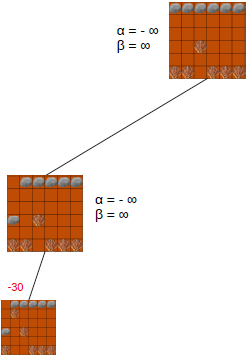
\includegraphics{img/ab1}
	\caption{Alpha-Beta Pruning: Schritt 1}
	\label{fig:ab1}
\end{figure}

\begin{figure}[h]
	\centering
	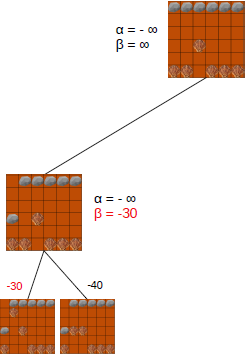
\includegraphics{img/ab2}
	\caption{Alpha-Beta Pruning: Schritt 2}
	\label{fig:ab2}
\end{figure}

\begin{figure}[h]
	\centering
	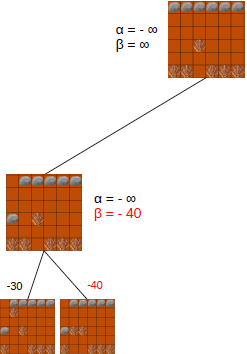
\includegraphics{img/ab3}
	\caption{Alpha-Beta Pruning: Schritt 3}
	\label{fig:ab3}
\end{figure}

\begin{figure}[h]
	\centering
	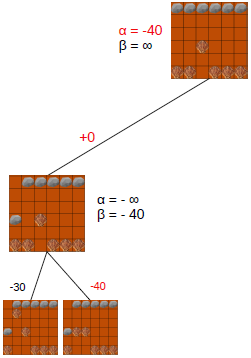
\includegraphics{img/ab4}
	\caption{Alpha-Beta Pruning: Schritt 4}
	\label{fig:ab4}
\end{figure}

\begin{figure}[h]
	\centering
	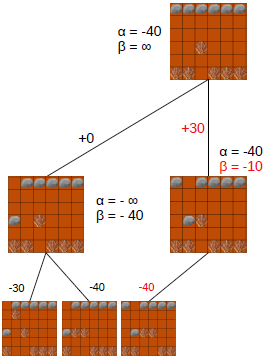
\includegraphics{img/ab5}
	\caption{Alpha-Beta Pruning: Schritt 5}
	\label{fig:ab5}
\end{figure}

\begin{figure}[h]
	\centering
	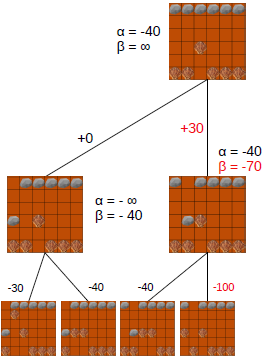
\includegraphics{img/ab6}
	\caption{Alpha-Beta Pruning: Schritt 6}
	\label{fig:ab6}
\end{figure}

\begin{figure}[h]
	\centering
	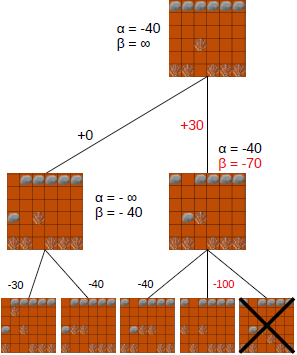
\includegraphics{img/ab7}
	\caption{Alpha-Beta Pruning: Schritt 7}
	\label{fig:ab7}
\end{figure}
\begin{figure}[h]
	\centering
	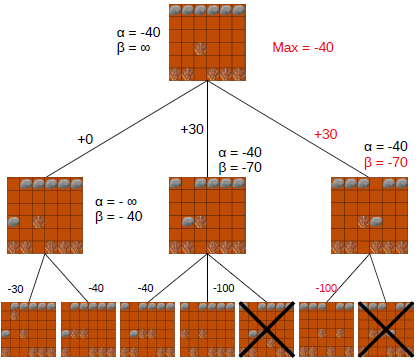
\includegraphics{img/ab8}
	\caption{Alpha-Beta Pruning: Schritt 8}
	\label{fig:ab8}
\end{figure}
%Diese Verbesserung wird dadurch erzielt, dass die Suche eines Pfades abgebrochen wird, sobald klar wird, dass das Ergebnis nicht beeinflusst wird. Als Beispiel kann die Abbildung 2.6 wieder betrachtet werden. Hier wird der linke Teilbaum zuerst durchsucht. Da jeweils vom besten Zug der Spieler ausgegangen wird, wird dieser Teilbaum durchsucht und beta wird anschließend auf -40 gesetzt (bester Zug der Muscheln). Anschließend wird der mittlere Teilbaum betrachtet. Hier wird der beste Zug der Muscheln mit -100 bewertet und somit eine neue untere Schranke von -100 festgelegt und die Durchsuchung der anderen Pfade abgebrochen, da eine bessere Wertung nicht erreichbar ist. Außerdem wird alpha mit +30 belegt. der letzte Teilbaum wird ebenfalls durchsucht bis die -100 getroffen wird und hier abgebrochen. Dadurch wird die Laufzeit verringert aber das selbe Endergebnis erzielt.



%%% Local Variables: 
%%% mode: latex
%%% TeX-master: "thesis"
%%% End: 
% Mögliche Erweiterungen
%% zusammenf.tex
%% $Id: zusammenf.tex 61 2012-05-03 13:58:03Z bless $
%%

\chapter{Diskussion und Ausblick}
\label{ch:fazit}
%% ==============================

(Keine Untergliederung mehr)

%%% Local Variables: 
%%% mode: latex
%%% TeX-master: "thesis"
%%% End: 
   	  % Diskussion und Ausblick

%% ++++++++++++++++++++++++++++++++++++++++++
%% Anhang
%% ++++++++++++++++++++++++++++++++++++++++++

\appendix
%\include{anhang_a}
%\include{anhang_b}

%% ++++++++++++++++++++++++++++++++++++++++++
%% Literatur
%% ++++++++++++++++++++++++++++++++++++++++++
%  mit dem Befehl \nocite werden auch nicht 
%  zitierte Referenzen abgedruckt

\cleardoublepage
\phantomsection
\addcontentsline{toc}{chapter}{\bibname}
%%
%\nocite{Ulrich Schadler. Latrunculi  ein verlorenes strategisches Brettspiel der Rmer. HOMO LUDENS  Der spielende Mensch,} % nur angeben, wenn auch nicht im Text zitierte Quellen 
           % erscheinen sollen
%\bibliographystyle{itmabbrv} % mit abgekürzten Vornamen der Autoren
%\bibliographystyle{plain} % abbrvnat unsrtnat
%\bibliographystyle{babplain-lf}
\bibliographystyle{abbrvdin}
% spezielle Zitierstile: Labels mit vier Buchstaben und Jahreszahl
%\bibliographystyle{itmalpha}  % ausgeschriebene Vornamen der Autoren
\bibliography{thesis}

%% ++++++++++++++++++++++++++++++++++++++++++
%% Index
%% ++++++++++++++++++++++++++++++++++++++++++
\ifnotdraft{
\cleardoublepage
\phantomsection
\printindex            % Index, Stichwortverzeichnis
}

 %
 % Die folgende Erklärung ist für Diplomarbeiten Pflicht
 % (siehe Prüfungsordnung), für Studienarbeiten nicht notwendig
 \thispagestyle{empty}
%\vspace*{35\baselineskip}
%\hbox to \textwidth{\hrulefill}
\par
\chapter*{Eidesstattliche Erklärung}

Hiermit erkläre ich, dass ich diese Bachelor-/Masterarbeit selbständig verfasst und keine anderen als die angegebenen Quellen und Hilfsmittel benutzt und die aus fremden Quellen direkt oder indirekt übernommenen Gedanken als solche kenntlich gemacht habe. Die Arbeit habe ich bisher keinem anderen Prüfungsamt in gleicher oder vergleichbarer Form vor-gelegt. Sie wurde bisher auch nicht veröffentlicht.

Trier, den xx. Monat 20xx

%%%%%%%%%%%%%%%%%%%%%%%%%%%%%%%%%%%%%%%%%%%%%%%%%%%%%%%%%%%%%%%%%%%%%%%%
%% Hinweis:
%%
%% Diese Erklärung wird von der Prüfungsordnung für Diplomarbeiten 
%% verlangt und ist zu unterschreiben. Für Studienarbeiten ist diese
%% Erklärung nicht zwingend notwendig, schadet aber auch nicht.
%%%%%%%%%%%%%%%%%%%%%%%%%%%%%%%%%%%%%%%%%%%%%%%%%%%%%%%%%%%%%%%%%%%%%%%%
\clearpage







 \blankpage % Leerseite auf Erklärungsrückseite
 
\end{document}
%% end of file
